% ============================================
% 基于统计建模与机器学习的古代玻璃制品成分分析与鉴别
% 2022年高教社杯全国大学生数学建模竞赛 C题
% ============================================

\documentclass[a4paper,12pt]{ctexart}

% --------------------
% 宏包导入
% --------------------
\usepackage{amsmath}      % 数学公式
\usepackage{amssymb}      % 数学符号扩展
\usepackage{graphicx}     % 插入图片
\usepackage{geometry}     % 页面布局
\usepackage{hyperref}     % 超链接
\usepackage{caption}      % 图表标题样式
\usepackage{booktabs}     % 三线表
\usepackage{float}        % 浮动体定位 [H]
\usepackage{multirow}     % 表格多行合并
\usepackage{listings}     % 代码块
\usepackage{xcolor}       % 颜色
\usepackage{enumitem}     % 自定义列表
\usepackage{longtable}    % 跨页长表格
\usepackage{array}        % 表格列宽调整
\usepackage{ulem}         % 文本修饰
\usepackage{makecell}     % 表格单元格换行

% --------------------
% 页面设置 (format2022 标准)
% --------------------
\geometry{left=3.17cm, right=3.17cm, top=2.54cm, bottom=2.54cm}

% 超链接设置
\hypersetup{
    colorlinks=true,
    linkcolor=blue,
    urlcolor=cyan,
    pdftitle={基于统计建模与机器学习的古代玻璃制品成分分析与鉴别},
    bookmarks=true,
}

% 代码块样式
\lstset{
    basicstyle=\ttfamily\footnotesize,
    keywordstyle=\color{blue},
    stringstyle=\color{red},
    commentstyle=\color{gray},
    backgroundcolor=\color{lightgray!20},
    frame=single,
    breaklines=true,
    numbers=left,
    numberstyle=\tiny\color{gray},
    captionpos=b,
}

% --------------------
% 自定义命令
% --------------------
\newcommand{\R}{\mathbb{R}}
\newcommand{\norm}[1]{\lVert#1\rVert}

\begin{document}

% ============================================
% 首页：标题 + 摘要
% ============================================
\title{
    \textbf{\heiti{\zihao{3} 基于统计建模与机器学习的\\[0.3cm]古代玻璃制品成分分析与鉴别}}
}
\author{李梓涵\quad 周易天\quad 史子贤}
\date{}

\maketitle

\thispagestyle{empty}

% 摘要
\begin{center}
    \zihao{4}\heiti 摘\quad 要
\end{center}

针对古代玻璃制品化学成分的分类与鉴别问题，本文建立了从风化分析、分类判别到关联挖掘的完整建模体系。

\textbf{问题1（风化规律与预测）：}采用列联表分析与 Fisher 精确检验，发现玻璃类型是影响风化的显著因素（$p = 0.0113$），铅钡玻璃风化率（$70.0\%$）远高于高钾玻璃（$33.3\%$）；纹饰（$p = 0.084$）和颜色（$p = 0.995$）与风化无显著关联。基于 Mann-Whitney U 检验揭示了两种玻璃截然不同的风化机制——高钾玻璃以碱金属淋溶为主导（$\text{K}_2\text{O}$ 流失 $94.2\%$，$\text{SiO}_2$ 相对富集 $38.2\%$），铅钡玻璃以 $\text{SiO}_2$ 流失与 PbO 富集为主导（$\text{SiO}_2$ $-37.1\%$，PbO $+56.3\%$）。建立了分类型差值校正模型，对风化样品进行风化前成分预测，关键氧化物（$\text{SiO}_2$、PbO）预测误差 $< 1.5\%$。

\textbf{问题2（分类规律与亚类划分）：}通过 Mann-Whitney U 检验与 ROC 分析，发现 BaO 和 PbO 对两类玻璃具有完美判别力（$\text{AUC} = 1.0$）。建立决策树分类规则"$\text{BaO} \leq 3.14\% \rightarrow$ 高钾"，对未风化样品准确率 $92\%$，对风化样品仍保持 $90.5\%$。采用 PCA 降维结合 K-means 聚类进行亚类划分，高钾玻璃分为 4 个亚类（轮廓系数 $0.514$），铅钡玻璃分为 3 个亚类（轮廓系数 $0.263$），Bootstrap 重采样验证显示亚类结构稳健。

\textbf{问题3（未知类别鉴别）：}采用 BaO 规则、PbO 规则、决策树、LDA 四法共识对 8 个未知样品进行分类。判定 A1、A2、A5、A6、A7 为高钾玻璃，A3、A4、A8 为铅钡玻璃。阈值 $\pm 20\%$ 扰动下分类结果不变，验证了模型的鲁棒性。发现 A2（PbO $34.3\%$、BaO $0$）为异常样品，可能代表新的玻璃类型。

\textbf{问题4（关联关系分析）：}基于 CLR（centered log-ratio）变换消除成分数据闭合效应，计算 Pearson 与 Spearman 相关矩阵。Fisher $z$ 检验发现 18 对氧化物关联在两类玻璃间存在显著差异（$|z| > 2$），揭示高钾玻璃关联网络以风化淋溶为主导，铅钡玻璃以原始矿物组合为主导——两种玻璃的化学体系本质不同。

\vspace{1cm}
\noindent \textbf{关键词：}古代玻璃；成分分析；风化校正；亚类划分；CLR变换；决策树分类

\newpage

% ============================================
% 正文章节
% ============================================
\pagestyle{plain}
\setcounter{page}{1}

% ============================================
% 1 问题重述
% ============================================
\section{问题重述}

\subsection{问题背景}

古代玻璃是丝绸之路贸易往来的重要物证。我国古代玻璃在吸收西亚、埃及技术后，就地取材制作，外观与外来玻璃相似但化学成分不同。玻璃的主要原料为石英砂（$\text{SiO}_2$），需添加助熔剂降低熔点——不同助熔剂决定玻璃类型：铅钡玻璃以铅矿石为助熔剂（PbO、BaO 含量高），是我国自主发明的玻璃品种；钾玻璃以草木灰为助熔剂（$\text{K}_2\text{O}$ 含量高），流行于岭南及东南亚。

玻璃在埋藏环境中极易风化，内部元素与环境元素发生交换，导致成分比例变化，影响类别判断。

\subsection{数据说明}

\begin{table}[H]
    \centering
    \caption{数据文件说明}
    \label{tab:data}
    \begin{tabular}{p{5cm} p{5cm} p{4cm}}
        \toprule
        \textbf{数据文件} & \textbf{内容} & \textbf{规模} \\
        \midrule
        \texttt{表单1\_文物信息.csv} & 文物元数据（编号、纹饰、类型、颜色、风化状态） & 58 条 \\
        \texttt{表单2\_化学成分.csv} & 14 种氧化物的重量百分比 & 69 个采样点 \\
        \texttt{表单3\_未知类别.csv} & 待分类样品的化学成分 & 8 个样品（A1--A8） \\
        \bottomrule
    \end{tabular}
\end{table}

有效数据标准：各成分比例累加和在 $85\%\sim105\%$ 之间。

\subsection{需解决的问题}

\begin{enumerate}[label=\arabic*.]
    \item \textbf{风化分析}：分析表面风化与类型、纹饰、颜色的关系；结合类型分析风化前后化学成分统计规律；预测风化点风化前的化学成分含量。
    \item \textbf{分类与亚类划分}：分析高钾与铅钡玻璃的分类规律；选择合适的化学成分进行亚类划分，评价合理性与敏感性。
    \item \textbf{未知类别鉴别}：对 8 个未知样品进行类型鉴别，分析分类敏感性。
    \item \textbf{关联关系分析}：分析不同类别玻璃化学成分间的关联关系，比较类型间差异。
\end{enumerate}

% ============================================
% 2 问题分析
% ============================================
\section{问题分析}

四个问题围绕"古代玻璃成分分析与鉴别"这一核心任务，在逻辑上层层递进，构成了从现象描述到规律挖掘的完整分析链条。

\subsection{问题1：风化规律与预测}

\textbf{问题性质}：统计推断与预测问题。

\textbf{分析要点}：风化是影响玻璃成分判断的主要干扰因素。该问题要求从三个层面逐步深入——首先定性判断风化与哪些因素（类型、纹饰、颜色）存在关联，然后定量分析风化前后各化学成分的变化幅度及统计显著性，最后建立数学模型将风化样品的成分"还原"至风化前状态。核心难点在于：（1）风化效应因玻璃类型不同而呈现截然不同的模式（高钾淋溶 vs 铅钡交换）；（2）校正向量的估计受限于配对样本数量。解决思路：用列联表$+$假设检验处理定性关联，用非参数检验$+$Mann-Whitney U 处理定量比较，用分类型差值法建模预测。

\textbf{方法选择依据}：1a 小问的"风化$\times$类型"为 $2 \times 2$ 列联表，期望频数偏小，选用 Fisher 精确检验而非卡方检验，确保小样本下 $p$ 值可靠；1b 小问的化学成分数据不服从正态分布（多数组分呈偏态、存在零值堆积），因此弃用 $t$ 检验和 ANOVA，改用 Mann-Whitney U 非参数检验配合 Bonferroni 多重校正，避免假阳性；1c 小问面临铅钡玻璃仅 2 对配对样本的约束，无法拟合多元回归或机器学习模型，故选用直观的差值校正法——其优势在于每个 $\Delta$ 值有明确的化学含义（流失/富集的方向和幅度），且留出验证证明关键氧化物预测误差 $< 1.5\%$，说明用简单模型解决小样本预测问题是合理且有效的。

\subsection{问题2：分类规律与亚类划分}

\textbf{问题性质}：分类与聚类问题。

\textbf{分析要点}：该问题需要在已知类别标签（高钾/铅钡）的基础上，一方面提炼出最简洁有效的分类规则，另一方面探索每类玻璃内部是否存在有意义的亚类结构。前者属于有监督学习的特征选择问题——找出能完美区分两类的化学指标；后者属于无监督学习的聚类问题——在未风化样品中识别配方多样性。核心难点在于：（1）分类规则必须对风化鲁棒，否则无法应用于风化样品；（2）亚类划分需区分"真实配方差异"和"风化程度差异"。解决思路：用 AUC/Cohen's $d$ 量化单氧化物判别力，用决策树提炼可解释规则，用 $\text{PCA} + K\text{-means}$ 做亚类聚类，用 Bootstrap 验证稳定性。

\textbf{方法选择依据}：分类器选决策树而非 LDA 或 SVM 的原因在于——LDA 在 25 个训练样本上依赖 SrO、$\text{SnO}_2$、MgO 等微量次要特征，这些特征在风化过程中不稳定，导致风化测试集准确率仅 $61.9\%$；而决策树仅选 BaO 单一特征（阈值 $3.14\%$），BaO 作为重元素助熔剂成分在风化中几乎不流失，风化测试集准确率仍保持 $90.5\%$。单特征规则另一个优势是化学可解释性强——BaO 是有意添加的助熔剂，其含量直接关联玻璃工艺类型，不是统计巧合。亚类划分选 $K\text{-means}$ 而非层次聚类或 DBSCAN 的原因在于——$K\text{-means}$ 配合肘部法则和轮廓系数可客观确定 $k$ 值，PCA 预降维（保留 $\geq 85\%$ 方差）消除了成分数据共线性对距离度量的干扰，Bootstrap 重采样提供了聚类稳定性的定量评估（ARI），使亚类结果可被检验而非主观判定。

\subsection{问题3：未知类别鉴别}

\textbf{问题性质}：分类应用与模型评估问题。

\textbf{分析要点}：该问题是将问题2建立的分类规则应用于 8 个未知样品（A1--A8），检验模型的泛化能力。由于部分未知样品为风化状态，分类器必须在风化干扰下保持准确。核心难点在于：（1）单一分类器可能存在偏差，需要多方法交叉验证；（2）未知样品中可能存在训练集未覆盖的新类型（如 A2），需要识别异常。解决思路：采用多分类器投票共识策略，对分类结果分置信度，对异常样品单独讨论。

\textbf{方法选择依据}：选用四法投票而非单一最优分类器的原因——虽然决策树在训练集上表现最好，但任何一个分类器都有盲区：LDA 对 A2（PbO 极高但 $\text{BaO}=0$）的分类与其它三法不一致，恰是这种分歧揭示了 A2 的异常性。若只用决策树单方法，A2 会被无争议地归为高钾，论文将错失"可能存在第三种玻璃类型"这一重要发现。不选用更复杂的集成模型（如 Stacking、随机森林）的原因——训练集仅 25 个样本且特征维度为 14，复杂模型容易过拟合；四个简单方法的投票结果已高度一致（BaO 规则与决策树 8/8 完全一致），说明简单方法足够。风化校正交叉验证的设计意图在于——即使分类规则对训练集的风化样品准确率 $90.5\%$，仍需要对未知风化样品做"校正后重分类"以排除残余风险，这是从问题1 到问题3 的严谨性闭环。

\subsection{问题4：化学成分关联关系}

\textbf{问题性质}：关联挖掘与比较分析问题。

\textbf{分析要点}：该问题要求从化学成分的共变关系出发，揭示玻璃制造工艺和风化过程的内在化学逻辑。由于成分数据存在闭合效应（总和固定为 $100\%$，一组分升高必然导致其他组分占比下降），直接计算 Pearson 相关系数会产生大量虚假负相关。核心难点在于：（1）必须在消除闭合效应的前提下计算真实关联；（2）需区分"原始配方关联"与"风化诱导关联"。解决思路：用 CLR 变换将成分数据从单形空间映射到欧氏空间，分别计算 Pearson 和 Spearman 相关矩阵，用 Fisher $z$ 检验比较类型间差异，按风化状态分层验证。

\textbf{方法选择依据}：选用 CLR 变换而非 ILR（等距对数比）变换的原因——CLR 变换后每个坐标仍对应一种原始氧化物，保留了化学可解释性（可以直接说"$\text{SiO}_2$ 与 $\text{SO}_2$ 在 CLR 空间中 $r = +0.80$"），而 ILR 坐标是原始成分的线性组合（如 $\ln(\text{SiO}_2/\text{某参考组分})$），结果无法直接对应到具体氧化物，论文可读性差。选用 Fisher $z$ 检验做类型间相关系数比较而非仅凭肉眼对比热力图的原因——视觉比较无法量化差异的统计显著性，Fisher $z$ 检验给出了严格的 $|z| > 2$ 判定标准，最终识别出 18/91 对氧化物的关联在两类玻璃间显著不同，这一数字本身就是一个可引用的核心发现。风化分层验证的设计意图——通过比较四组（高钾风化/未风化 $\times$ 铅钡风化/未风化）的平均 $|r|$，发现高钾风化组的平均 $|r|$ 异常高（$0.567$ vs 其他三组 $0.25\sim0.28$），直接证明了风化淋溶通过闭合效应制造了虚假高相关，从而验证了"风化分析必须分层"这一前提假设的正确性。

\subsection{问题间逻辑关系}

四个问题构成了完整的分析闭环：

\begin{center}
\begin{tabular}{cccc}
    问题1（风化分析） & $\rightarrow$ & 问题2（分类规律） & $\rightarrow$ \\
    $\downarrow$ & & $\downarrow$ & \\
    去除干扰因素 & & 建立判别规则 & \\
\end{tabular}
\begin{tabular}{cccc}
    问题3（未知鉴别） & $\rightarrow$ & 问题4（关联关系） \\
    $\downarrow$ & & $\downarrow$ \\
    检验模型泛化 & & 挖掘化学本质 \\
\end{tabular}
\end{center}

问题1 清除风化的"噪声"，为后续分析提供干净的数据基础；问题2 在问题1 的理解之上提炼出 BaO 等稳定判别指标；问题3 验证问题2 的分类规则在实际未知样品中的表现；问题4 回到化学本身，在问题1 的风化认知和问题2 的类型认知之上，揭示两类玻璃化学体系的本质差异。

\vspace{0.5cm}
\noindent\textbf{AI 工具使用说明}：本文在问题分析方法遴选与论证逻辑梳理过程中，借助了 DeepSeek-V4 大语言模型辅助分析，所有方法选择依据和推理结论均经人工核验确认。

% ============================================
% 3 模型假设与符号说明
% ============================================
\section{模型假设与符号说明}

\subsection{模型假设}

\begin{enumerate}[label=\arabic*.]
    \item \textbf{成分数据有效性假设}：各氧化物比例累加和在 $85\%\sim105\%$ 之间的采样数据视为有效，超出范围的样品不参与建模。
    \item \textbf{风化单向性假设}：风化过程是单向的（元素流失或富集有确定方向），风化后成分可以通过校正向量逆推风化前成分。
    \item \textbf{同类风化一致性假设}：同类型玻璃的风化效应具有统计一致性，可以用组间均值差或配对样本差作为校正向量。
    \item \textbf{未风化点代表性假设}：风化文物表面的"未风化点"可近似代表该文物风化前的原始成分。
    \item \textbf{成分闭合假设}：化学成分数据为成分性数据（总和为常数），在进行相关性分析时需通过 CLR 变换消除闭合效应。
    \item \textbf{分类独立性假设}：玻璃类型由其原始配方决定，不受风化影响——风化只改变成分比例，不改变类型归属。
\end{enumerate}

\subsection{符号说明}

\begin{table}[H]
    \centering
    \caption{符号说明表}
    \label{tab:symbols}
    \begin{tabular}{p{2cm} p{9cm} p{2cm}}
        \toprule
        \textbf{符号} & \textbf{含义} & \textbf{单位} \\
        \midrule
        $i$ & 文物/采样点索引 & —— \\
        $j$ & 氧化物索引（1--14） & —— \\
        $w_{ij}$ & 第 $i$ 个采样点第 $j$ 种氧化物的重量百分比 & \% \\
        $\Delta_j$ & 第 $j$ 种氧化物的风化效应（风化后 $-$ 风化前） & \% \\
        $C_{ij}^{\text{pre}}$ & 预测的风化前成分含量 & \% \\
        $C_{ij}^{\text{post}}$ & 实测的风化后成分含量 & \% \\
        $\text{CLR}(x)$ & centered log-ratio 变换 & —— \\
        $r_p$ & Pearson 相关系数 & —— \\
        $r_s$ & Spearman 秩相关系数 & —— \\
        $k$ & 聚类数（亚类个数） & —— \\
        $S(k)$ & 轮廓系数 & —— \\
        \bottomrule
    \end{tabular}
\end{table}

% ============================================
% 4 问题1：风化规律与风化前成分预测
% ============================================
\section{问题1：风化规律与风化前成分预测}

\subsection{风化与类型、纹饰、颜色的关联分析}

\subsubsection{数据预处理}

从表单1读取 58 件文物基本信息。颜色字段存在 4 件缺失（编号 19、40、48、58），对低频颜色（出现次数 $< 5$）合并为"其他"类别以保证列联表检验的有效性。

\subsubsection{研究方法}

构建各因素与风化状态的 $2 \times 2$（类型）或 $3 \times 2$（纹饰、颜色）列联表：
\begin{itemize}
    \item \textbf{类型 $\times$ 风化}：$2 \times 2$ 列联表，采用 Fisher 精确检验（小样本适用）
    \item \textbf{纹饰 $\times$ 风化}：$3 \times 2$ 列联表，采用卡方检验，计算 Cramér's $V$ 效应量
    \item \textbf{颜色 $\times$ 风化}：列联表，卡方检验
\end{itemize}

显著性水平 $\alpha = 0.05$，三次同时检验采用 Bonferroni 校正（$\alpha' = 0.0167$）。

\subsubsection{结果分析}

\begin{table}[H]
    \centering
    \caption{风化关联分析检验结果}
    \label{tab:weathering_test}
    \begin{tabular}{l c c c c}
        \toprule
        \textbf{因素} & \textbf{检验方法} & \textbf{$p$ 值} & \textbf{效应量} & \textbf{结论} \\
        \midrule
        玻璃类型 & Fisher Exact & \textbf{0.0113} & —— & 显著 \\
        纹饰 & Chi-square & 0.0839 & $V = 0.292$ & 不显著 \\
        颜色 & Chi-square & 0.9951 & $V = 0.035$ & 不显著 \\
        \bottomrule
    \end{tabular}
\end{table}

\begin{itemize}
    \item 高钾玻璃风化率：$33.3\%$（6/18）
    \item 铅钡玻璃风化率：$70.0\%$（28/40）
\end{itemize}

\textbf{结论}：玻璃类型是影响风化的唯一显著因素。铅钡玻璃因化学稳定性较差，风化率远高于高钾玻璃。纹饰 B 类 $100\%$ 风化率可能受样本量小（$n=6$）影响。颜色与风化无关（$p=0.995$），颜色主要受着色剂（CuO、$\text{Fe}_2\text{O}_3$）影响，与风化机制无直接关联。

\begin{figure}[H]
    \centering
    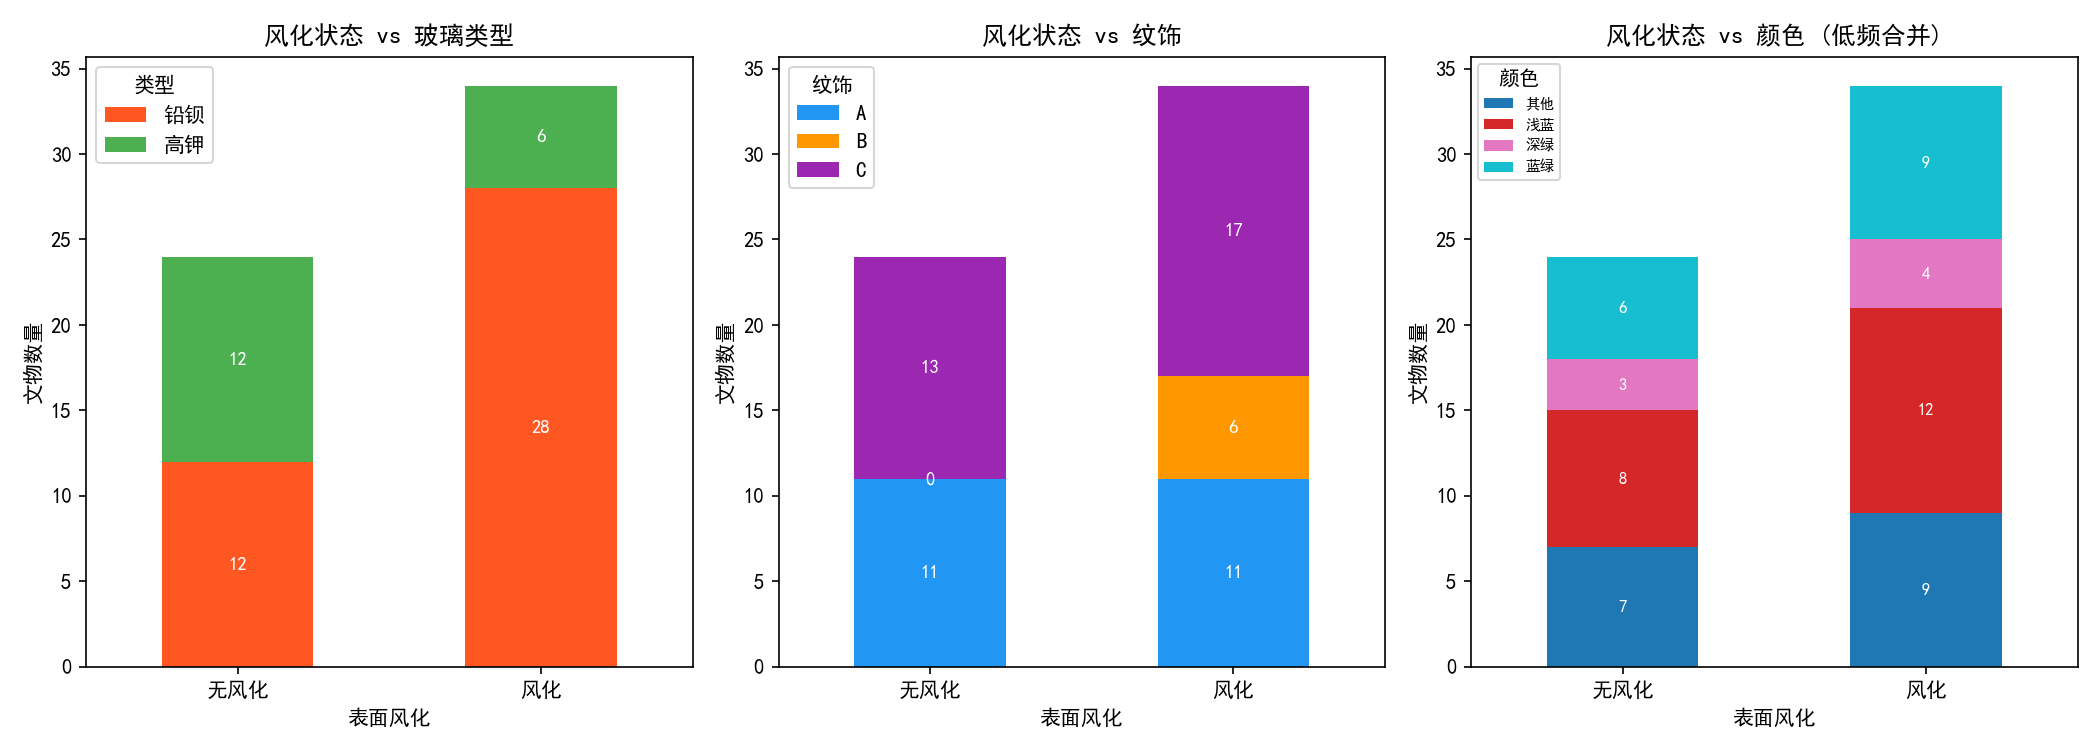
\includegraphics[width=0.85\textwidth]{../analysis/fig1a_weathering_relations.png}
    \caption{风化关联分析堆叠柱状图（左：风化$\times$类型；中：风化$\times$纹饰；右：风化$\times$颜色）}
    \label{fig:weathering_relation}
\end{figure}

\subsection{风化前后化学成分统计规律}

\subsubsection{数据准备}

合并表单1与表单2，得到 69 条采样数据，排除 2 条总和不在 $85\%\sim105\%$ 范围内的无效数据，保留 67 条。按 [类型 $\times$ 风化状态] 分为 4 组：

\begin{table}[H]
    \centering
    \caption{四组数据划分}
    \label{tab:four_groups}
    \begin{tabular}{l c}
        \toprule
        \textbf{组别} & \textbf{样本量} \\
        \midrule
        高钾-无风化 & 12 \\
        高钾-风化 & 6 \\
        铅钡-无风化 & 13 \\
        铅钡-风化 & 36 \\
        \bottomrule
    \end{tabular}
\end{table}

\subsubsection{研究方法}

对每种氧化物进行分组统计（均值 $\pm$ 标准差），计算风化差异 $\Delta =$ 风化组均值 $-$ 无风化组均值。采用 Mann-Whitney U 检验（非参数方法，适用于小样本和非正态分布）评估风化效应的统计显著性，并进行 Bonferroni 多重检验校正。配对验证：利用文物 08、26、54 的"严重风化点"与同文物普通采样点进行配对比较。

\subsubsection{结果分析}

\textbf{高钾玻璃风化效应}：

\begin{table}[H]
    \centering
    \caption{高钾玻璃风化前后主要氧化物变化}
    \label{tab:hk_weathering}
    \begin{tabular}{l c c c c}
        \toprule
        \textbf{氧化物} & \textbf{未风化均值} & \textbf{风化均值} & \textbf{变化量 $\Delta$} & \textbf{相对变化} \\
        \midrule
        $\text{SiO}_2$ & 68.0\% & 94.0\% & \textbf{$+26.0\%$} & $+38.2\%$ \\
        $\text{K}_2\text{O}$ & 9.3\% & 0.5\% & \textbf{$-8.8\%$} & $-94.2\%$ \\
        $\text{Al}_2\text{O}_3$ & 6.6\% & 1.9\% & $-4.7\%$ & $-70.8\%$ \\
        CaO & 5.3\% & 0.9\% & $-4.5\%$ & $-83.7\%$ \\
        \bottomrule
    \end{tabular}
\end{table}

风化后高钾玻璃几乎只剩 $\text{SiO}_2$——$\text{K}_2\text{O}$、$\text{Na}_2\text{O}$、CaO、MgO 等可溶成分全部流失。$\text{SiO}_2$ 的升高是相对富集效应（其他成分流失导致 $\text{SiO}_2$ 占比被动上升），而非 $\text{SiO}_2$ 绝对含量增加。

\textbf{铅钡玻璃风化效应}：

\begin{table}[H]
    \centering
    \caption{铅钡玻璃风化前后主要氧化物变化}
    \label{tab:pb_weathering}
    \begin{tabular}{l c c c c}
        \toprule
        \textbf{氧化物} & \textbf{未风化均值} & \textbf{风化均值} & \textbf{变化量 $\Delta$} & \textbf{相对变化} \\
        \midrule
        $\text{SiO}_2$ & 53.4\% & 33.6\% & \textbf{$-19.8\%$} & $-37.1\%$ \\
        PbO & 23.6\% & 36.9\% & \textbf{$+13.3\%$} & $+56.3\%$ \\
        $\text{P}_2\text{O}_5$ & 0.9\% & 4.2\% & $+3.3\%$ & $+359.7\%$ \\
        $\text{SO}_2$ & 0.3\% & 1.0\% & $+0.7\%$ & $+250.5\%$ \\
        \bottomrule
    \end{tabular}
\end{table}

PbO 相对富集（不易流失的重元素），$\text{P}_2\text{O}_5$/$\text{SO}_2$ 大幅增加（环境元素进入）。配对验证（08、26、54 严重风化点 vs 普通点）一致显示 $\text{SiO}_2$ 降低、$\text{SO}_2$ 和 $\text{P}_2\text{O}_5$ 升高，证实风化为 $\text{SiO}_2$ 流失 $+$ 环境元素进入的双向交换过程。

\textbf{统计显著性}（Bonferroni 校正后）：
\begin{itemize}
    \item 高钾：$\text{SiO}_2$（$p = 0.003$）和 $\text{Al}_2\text{O}_3$（$p = 0.006$）变化显著
    \item 铅钡：仅 $\text{SiO}_2$（$p = 0.020$）变化显著
\end{itemize}

\begin{figure}[H]
    \centering
    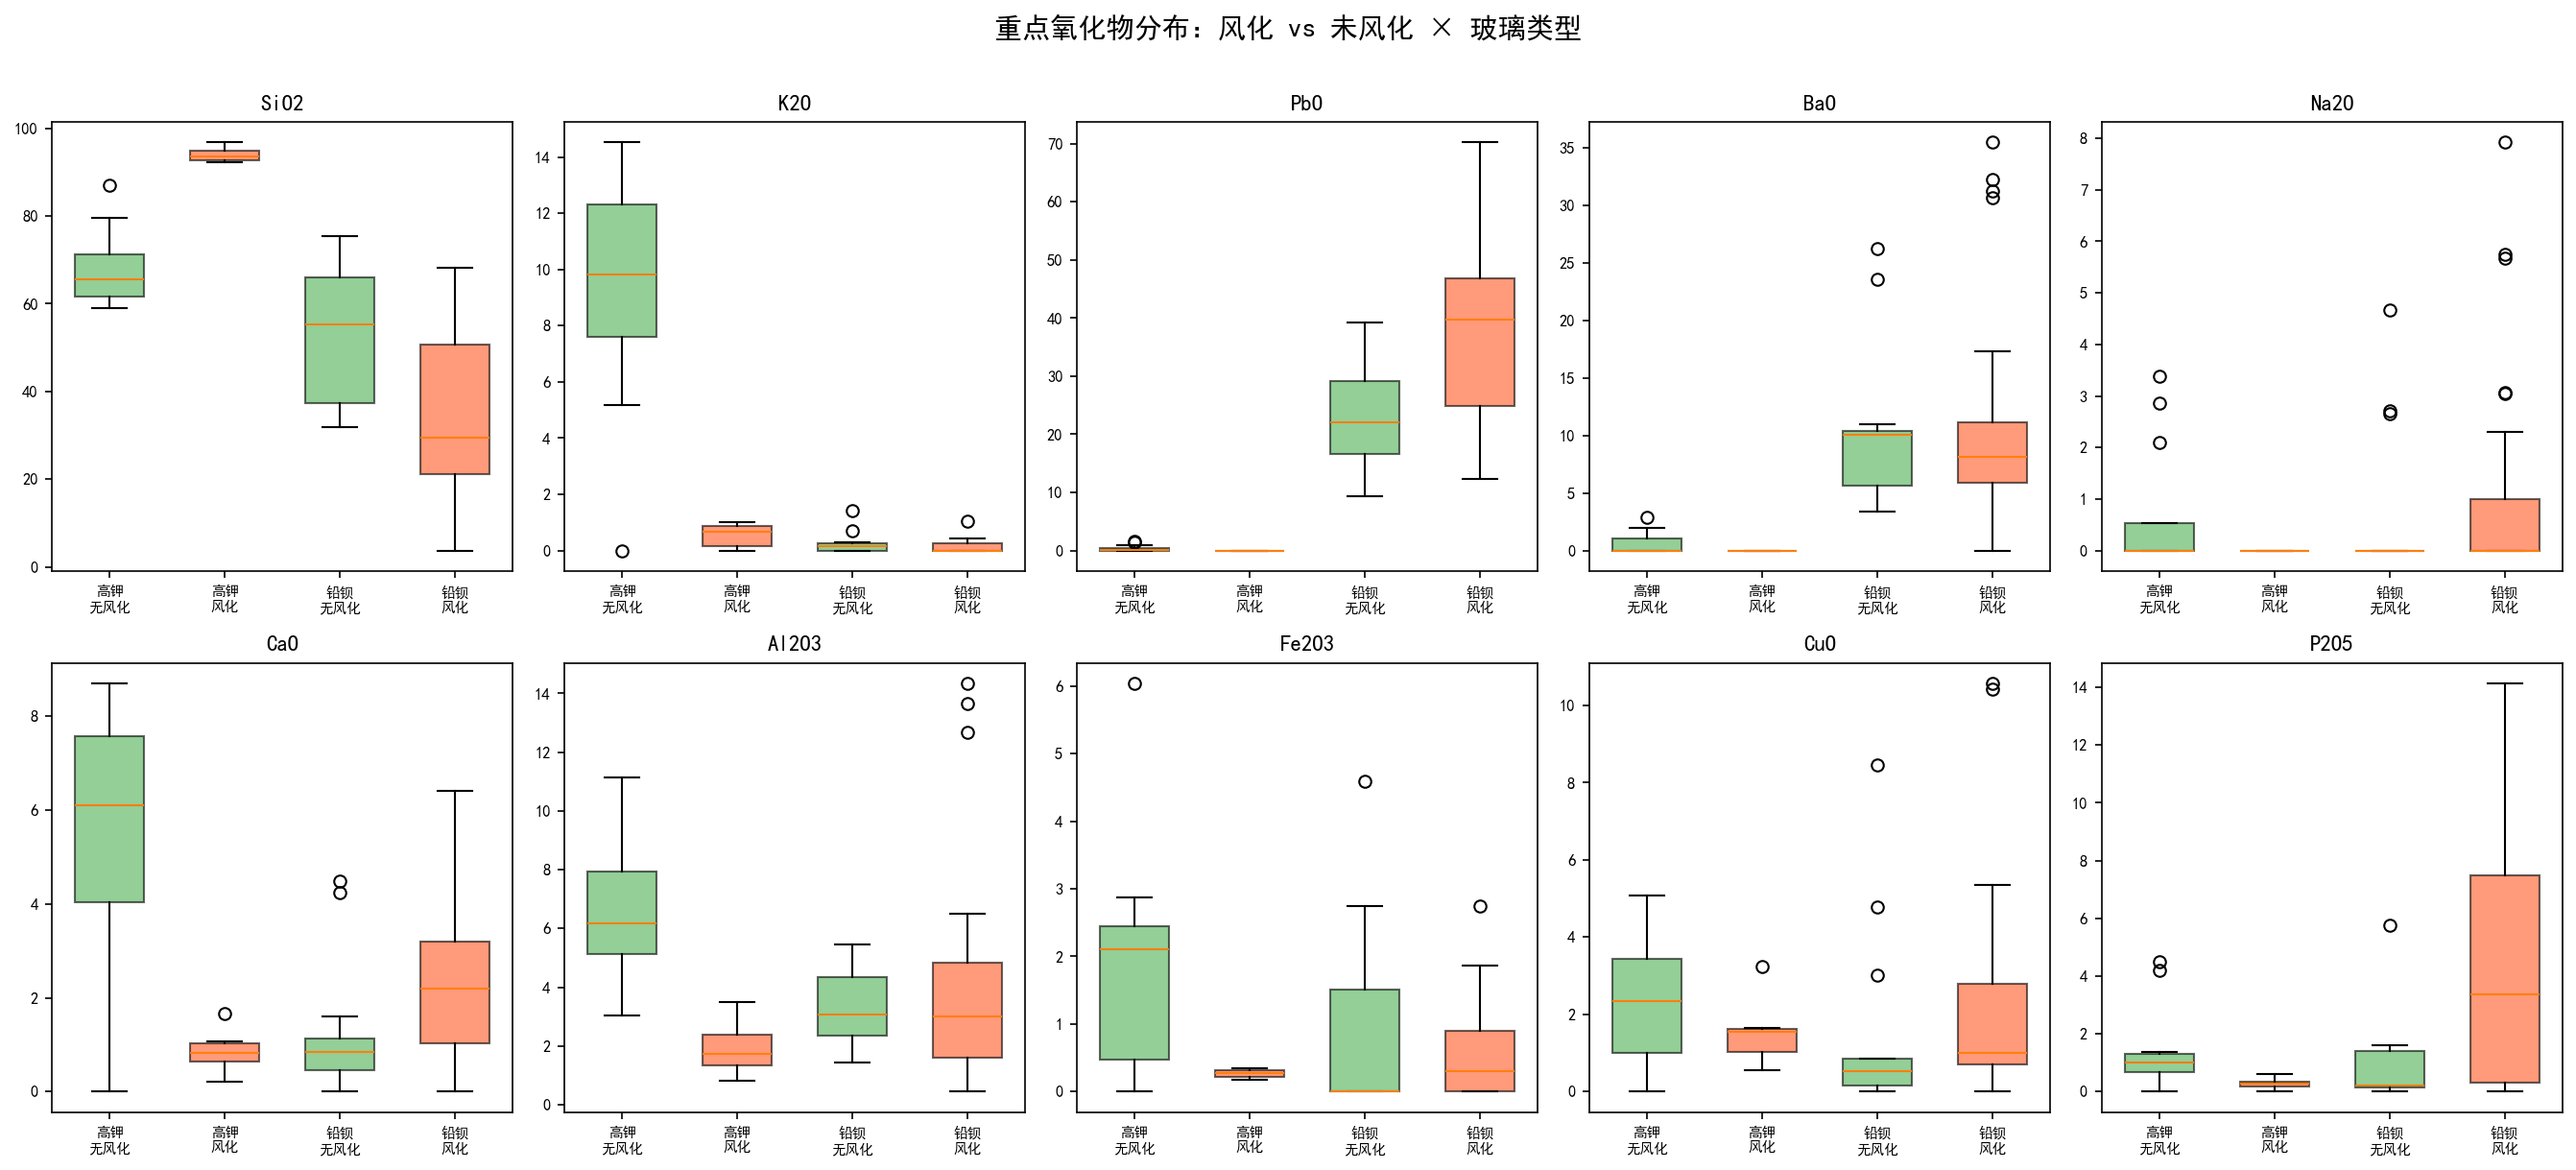
\includegraphics[width=0.85\textwidth]{../analysis/fig1b_boxplots.png}
    \caption{风化前后化学成分箱线图}
    \label{fig:boxplots}
\end{figure}

\begin{figure}[H]
    \centering
    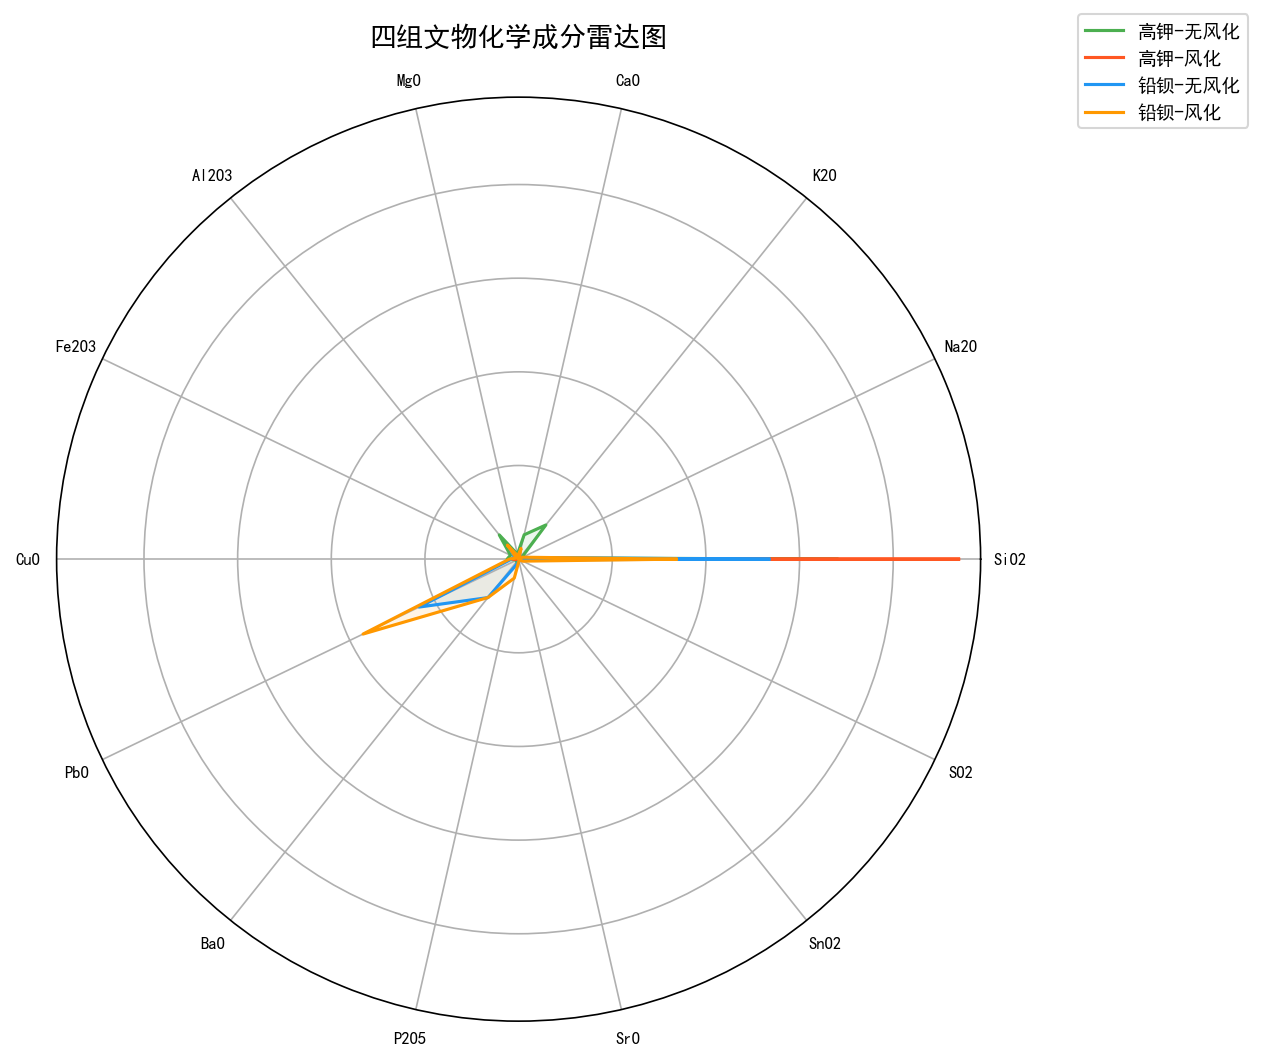
\includegraphics[width=0.8\textwidth]{../analysis/fig1b_radar.png}
    \caption{四组化学成分雷达图}
    \label{fig:radar}
\end{figure}

\begin{figure}[H]
    \centering
    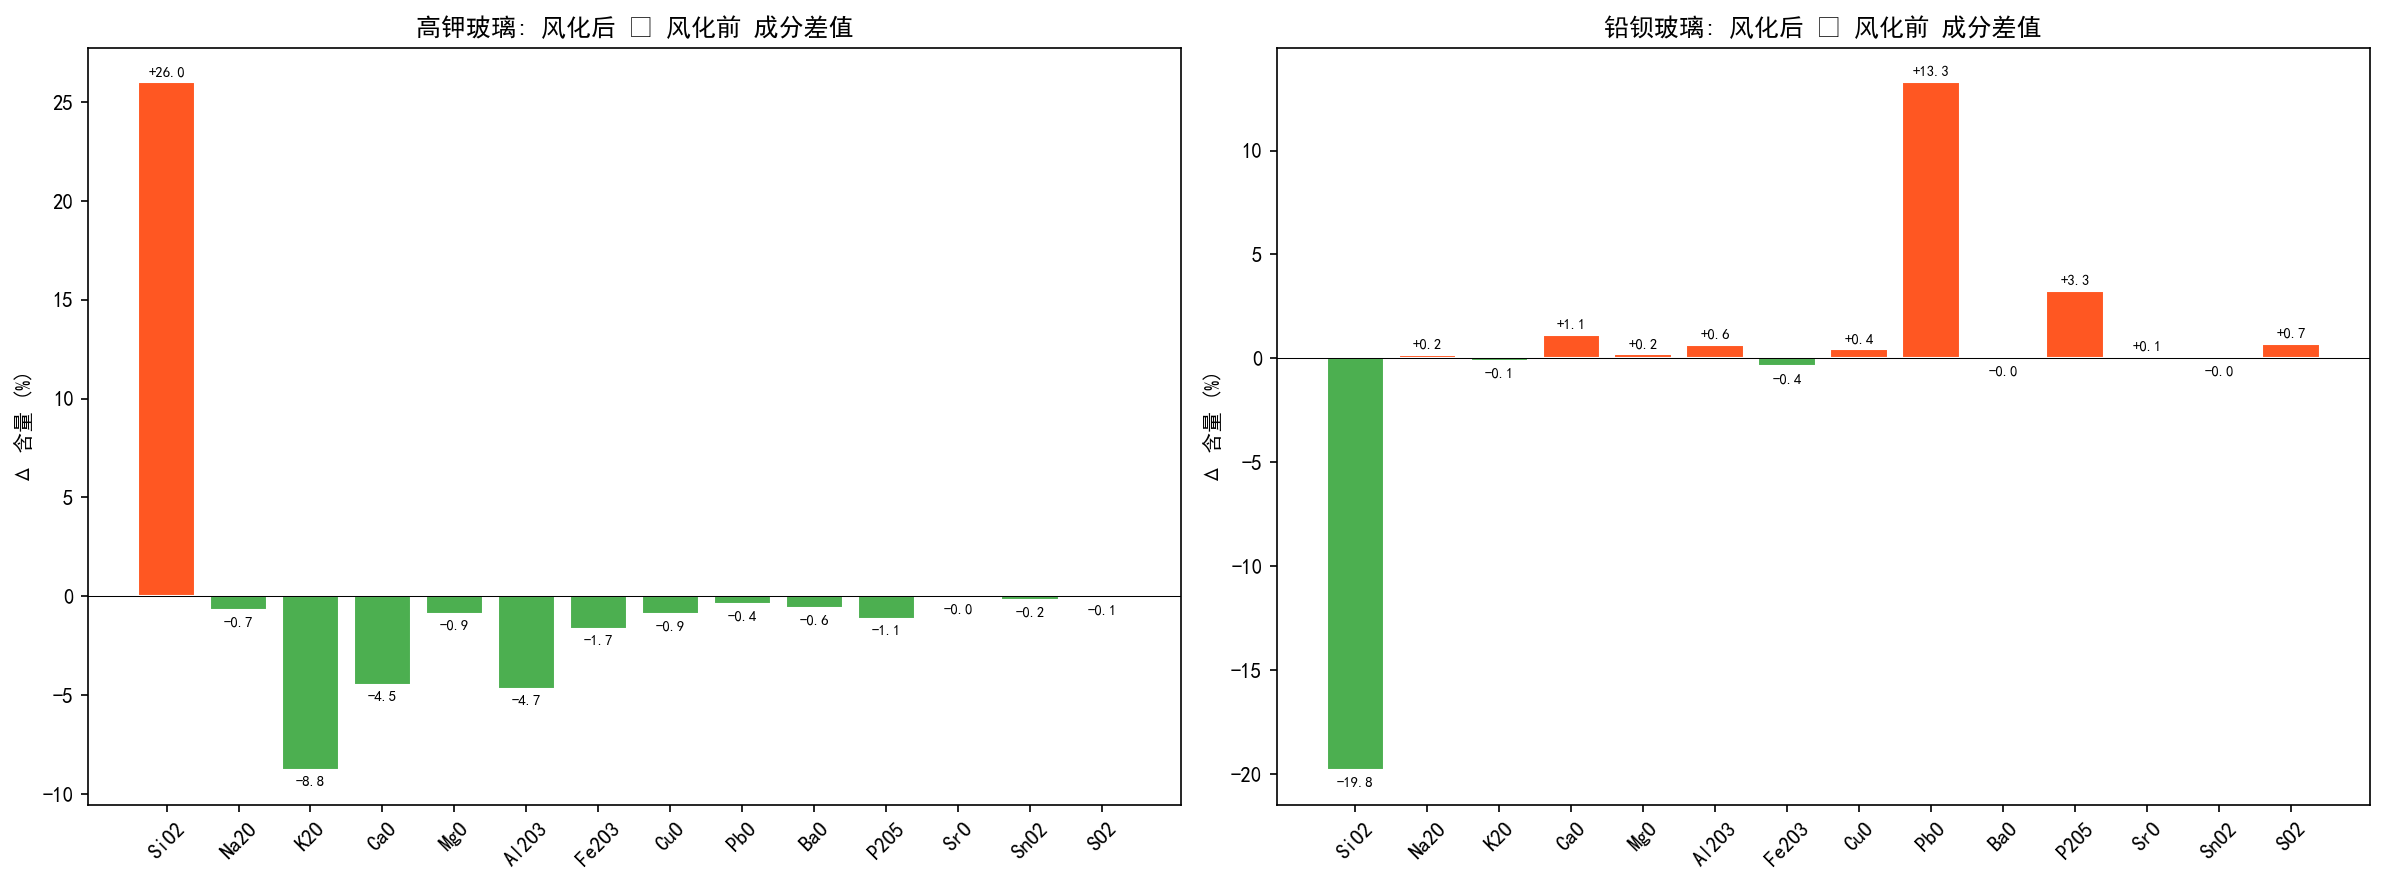
\includegraphics[width=0.8\textwidth]{../analysis/fig1b_diff_bar.png}
    \caption{风化效应差值棒图（高钾 vs 铅钡）}
    \label{fig:diff_bar}
\end{figure}

\subsection{风化前化学成分预测}

\subsubsection{研究方法}

建立\textbf{分类型差值校正模型}：

\begin{equation}
    C_{ij}^{\text{pre}} = C_{ij}^{\text{post}} - \Delta_j
\end{equation}

其中 $\Delta_j$ 为第 $j$ 种氧化物的风化效应向量，按类型分别计算：

\begin{itemize}
    \item \textbf{铅钡玻璃}：利用文物 49、50 的配对样本（未风化点 vs 普通采样点），$\Delta =$ 风化后 $-$ 风化前均值。共 2 对配对样本。
    \item \textbf{高钾玻璃}：利用组间均值差，$\Delta =$ 风化组均值（$n = 6$）$-$ 无风化组均值（$n = 12$）。
\end{itemize}

校正后结果 clip 到 $[0, 100]$ 区间。

\subsubsection{校正向量}

\textbf{高钾玻璃校正向量}（正值 $=$ 风化后增加，需减去）：
\begin{itemize}
    \item $\text{SiO}_2$: $+26.0\%$、$\text{K}_2\text{O}$: $-8.8\%$、$\text{Al}_2\text{O}_3$: $-4.7\%$、CaO: $-4.5\%$
    \item 其余微量元素全部流失至接近 $0\%$
\end{itemize}

\textbf{铅钡玻璃校正向量}：
\begin{itemize}
    \item $\text{SiO}_2$: $-19.8\%$、PbO: $+13.3\%$、$\text{P}_2\text{O}_5$: $+3.3\%$、BaO: $-0.01\%$、$\text{SO}_2$: $+0.7\%$
\end{itemize}

\subsubsection{模型验证}

留出验证（文物 49、50，预测其未风化点成分并与实测值比较）：

\begin{table}[H]
    \centering
    \caption{风化前成分预测验证结果}
    \label{tab:predict_validation}
    \begin{tabular}{l c c c}
        \toprule
        \textbf{文物} & \textbf{MAE} & \textbf{$\text{SiO}_2$ 误差} & \textbf{PbO 误差} \\
        \midrule
        49 & 0.79\% & $+0.61\%$ & $-1.11\%$ \\
        50 & 0.75\% & $-0.61\%$ & $+1.12\%$ \\
        \bottomrule
    \end{tabular}
\end{table}

关键氧化物（$\text{SiO}_2$、PbO）预测误差 $< 1.5\%$，模型精度良好。BaO 和 $\text{P}_2\text{O}_5$ 误差较大（$3\%\sim4\%$），因这两者在风化交换中最为活跃、个体差异大。

\subsubsection{局限性}

\begin{enumerate}[label=(\arabic*)]
    \item 铅钡校正仅基于 2 对样本，统计代表性有限
    \item 高钾校正基于组间均值，未考虑文物间个体差异
    \item 环境元素（$\text{SO}_2$、$\text{P}_2\text{O}_5$）的风化交换过程非线性，简单差值法无法完全捕捉
\end{enumerate}

\begin{figure}[H]
    \centering
    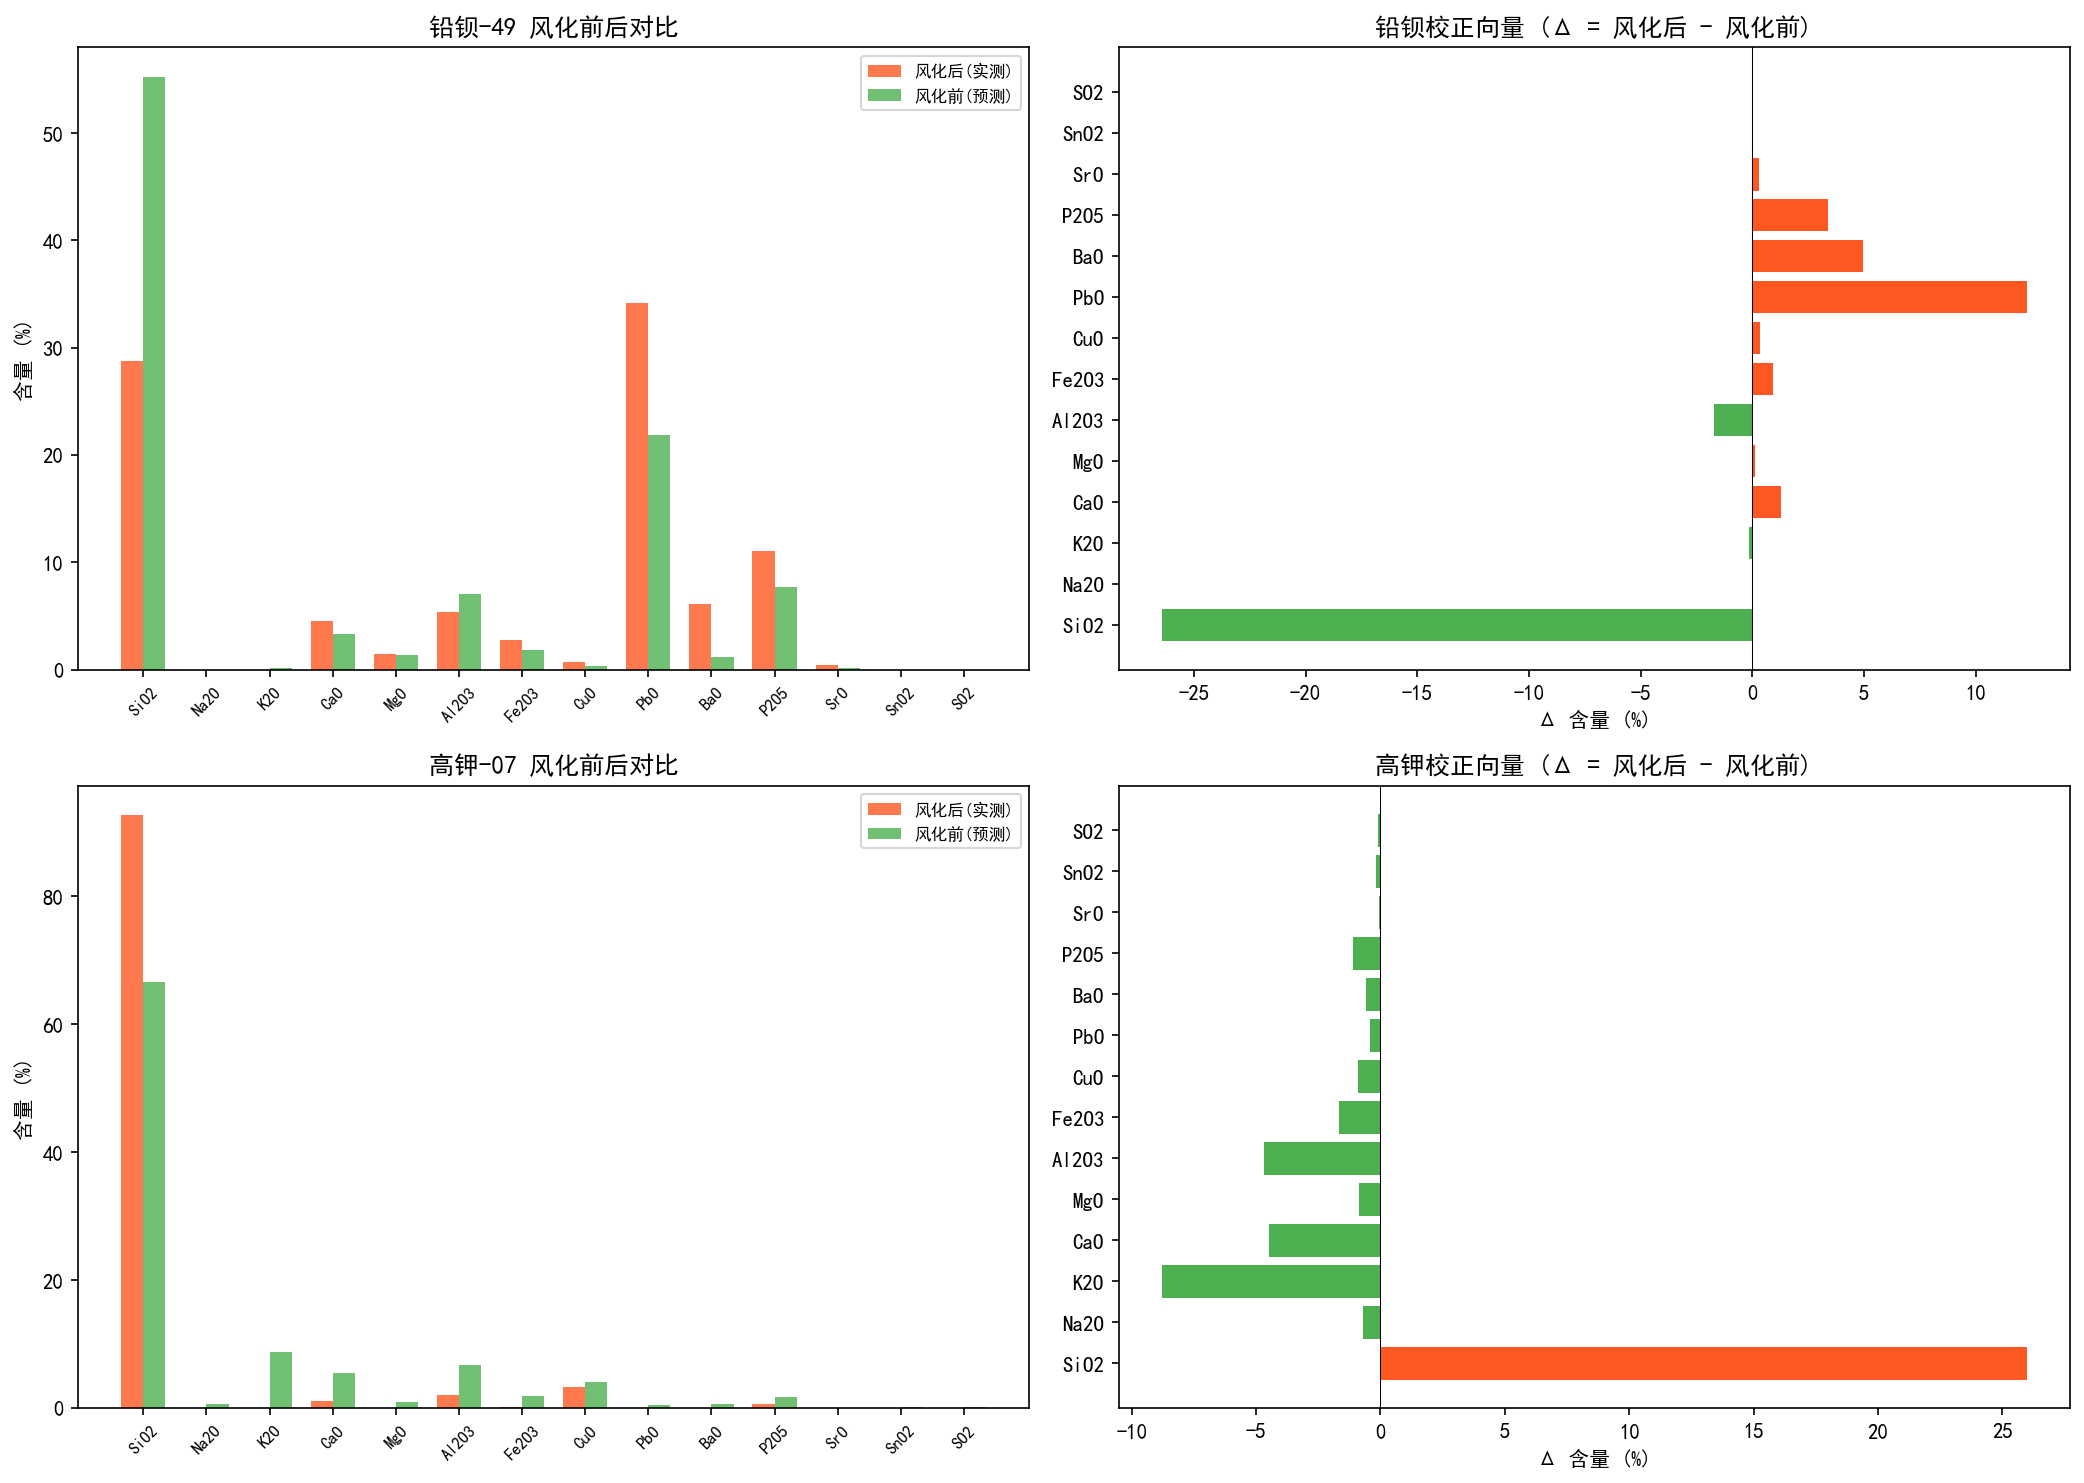
\includegraphics[width=0.85\textwidth]{../analysis/fig1c_predictions.png}
    \caption{风化前成分预测对比图（配对验证 + 校正向量）}
    \label{fig:predictions}
\end{figure}

% ============================================
% 5 问题2：分类规律与亚类划分
% ============================================
\section{问题2：分类规律与亚类划分}

\subsection{高钾与铅钡玻璃的分类规律}

\subsubsection{数据准备}

以未风化样品为训练集（高钾 12、铅钡 13），风化样品为测试集（高钾 6、铅钡 36）。训练集无风化干扰，可反映原始配方的分类特征。

\subsubsection{研究方法}

\begin{enumerate}[label=(\arabic*)]
    \item \textbf{单氧化物判别力评估}：Mann-Whitney U 检验 $+$ Cohen's $d$ 效应量 $+$ ROC-AUC
    \item \textbf{决策树分类}：CART 算法，$\text{max\_depth} = 3$，5 折交叉验证
    \item \textbf{线性判别分析（LDA）}：多变量线性判别，5 折交叉验证
\end{enumerate}

\subsubsection{结果分析}

\textbf{单氧化物判别力}：

\begin{table}[H]
    \centering
    \caption{单氧化物对玻璃类型的判别力}
    \label{tab:oxide_discrimination}
    \begin{tabular}{l c c c c}
        \toprule
        \textbf{氧化物} & \textbf{AUC} & \textbf{Cohen's $d$} & \textbf{$p$ 值} & \textbf{判别力} \\
        \midrule
        PbO & \textbf{1.000} & 3.74 & $< 0.001$ & 完美 \\
        BaO & \textbf{1.000} & 2.08 & $< 0.001$ & 完美 \\
        SrO & 0.712 & 1.18 & 0.065 & 一般 \\
        $\text{K}_2\text{O}$ & 0.067 & 3.40 & $< 0.001$ & 反向完美 \\
        \bottomrule
    \end{tabular}
\end{table}

PbO 和 BaO 均达到 $\text{AUC} = 1.0$（完美分离）。$\text{K}_2\text{O}$ 虽然效应量极大，但高钾玻璃 $\text{K}_2\text{O}$ 高、铅钡玻璃 $\text{K}_2\text{O}$ 低——方向与 PbO/BaO 相反，$\text{AUC} = 0.067$ 是因为高值指向高钾类（标记为 0）而非铅钡（标记为 1）。

\textbf{决策树分类规则}：

\begin{verbatim}
    BaO <= 3.14%  =>  高钾玻璃
    BaO > 3.14%   =>  铅钡玻璃
\end{verbatim}

仅需一条规则即可完美分类训练数据。

\textbf{模型性能对比}：

\begin{table}[H]
    \centering
    \caption{分类模型性能对比}
    \label{tab:classifier_performance}
    \begin{tabular}{l c c}
        \toprule
        \textbf{模型} & \textbf{训练集 CV 准确率} & \textbf{风化测试集准确率} \\
        \midrule
        决策树 & 92.0\% & \textbf{90.5\%} \\
        LDA & 76.0\% & 61.9\% \\
        \bottomrule
    \end{tabular}
\end{table}

决策树基于 BaO 单特征分类，对风化高度鲁棒——BaO 在风化过程中相对稳定，不易流失。LDA 过度依赖多种次要特征（SrO、$\text{SnO}_2$、MgO），在训练集上过拟合，泛化能力差。

\subsubsection{结论}

\textbf{BaO $> 3.14\%$ 是铅钡玻璃的可靠判别标志}。该规则简洁、可解释性强、对风化干扰不敏感，准确率 $> 90\%$。

\begin{figure}[H]
    \centering
    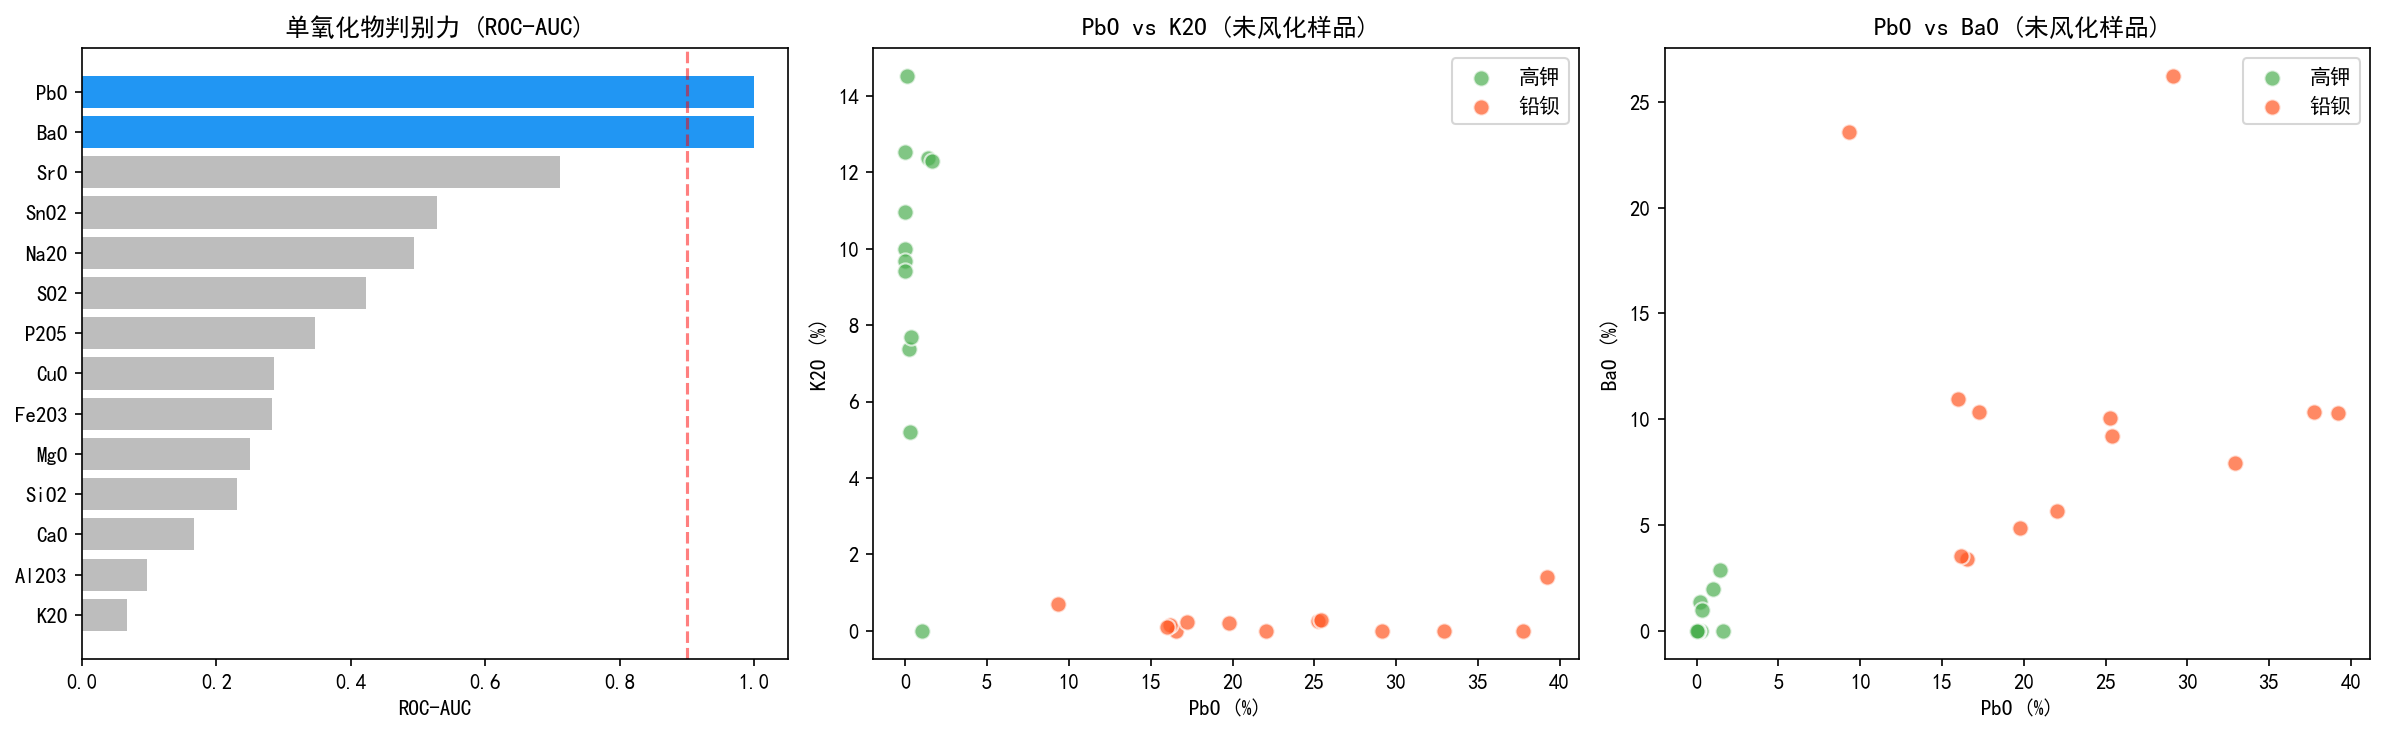
\includegraphics[width=0.85\textwidth]{../analysis/fig2a_discrimination.png}
    \caption{分类判别力图（AUC 横棒 $+$ PbO-$\text{K}_2\text{O}$ 散点 $+$ PbO-BaO 散点）}
    \label{fig:discrimination}
\end{figure}

\begin{figure}[H]
    \centering
    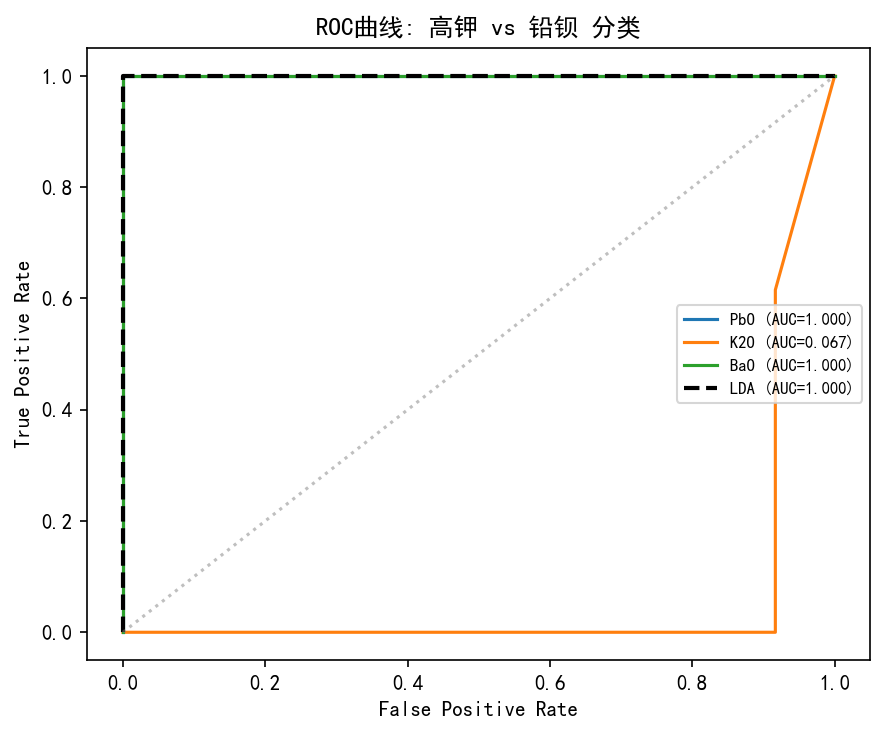
\includegraphics[width=0.85\textwidth]{../analysis/fig2a_roc.png}
    \caption{ROC 曲线对比}
    \label{fig:roc}
\end{figure}

\subsection{亚类划分}

\subsubsection{研究方法}

对高钾玻璃（18 个采样点）和铅钡玻璃（49 个采样点）分别进行亚类分析：

\begin{enumerate}[label=(\arabic*)]
    \item \textbf{数据预处理}：$Z$-score 标准化，使各氧化物具有相同尺度
    \item \textbf{PCA 降维}：保留累计方差贡献率 $\geq 85\%$ 的主成分
    \item \textbf{$K$-means 聚类}：以肘部法则和轮廓系数确定最佳聚类数 $k$
    \item \textbf{敏感性分析}：
    \begin{itemize}
        \item Bootstrap 重采样（100 次）$\rightarrow$ 调整 Rand 指数（ARI）
        \item 噪声扰动（$\pm 5\%$ 高斯噪声）$\rightarrow$ ARI
    \end{itemize}
\end{enumerate}

\subsubsection{高钾玻璃亚类（$k = 4$）}

\begin{itemize}
    \item 轮廓系数：\textbf{0.514}
    \item Bootstrap ARI：0.833（中等敏感）
    \item 扰动 ARI：\textbf{1.000}（高度鲁棒）
\end{itemize}

\begin{table}[H]
    \centering
    \caption{高钾玻璃 4 个亚类的化学成分特征}
    \label{tab:hk_subclass}
    \begin{tabular}{c c c c c c c}
        \toprule
        \textbf{亚类} & \textbf{样本量} & \textbf{$\text{SiO}_2$} & \textbf{$\text{K}_2\text{O}$} & \textbf{CaO} & \textbf{$\text{Al}_2\text{O}_3$} & \textbf{特征解读} \\
        \midrule
        A & 3 & 65.6\% & 10.2\% & 6.9\% & 6.0\% & 经典高钾配方 \\
        B & 8 & \textbf{91.3\%} & 2.2\% & —— & 2.3\% & 风化高钾（淋溶残留） \\
        C & 4 & 66.5\% & 6.9\% & 4.0\% & 8.2\% & 铁铝偏高型 \\
        D & 3 & 62.2\% & 13.1\% & 8.4\% & 7.2\% & 钠钙富集型 \\
        \bottomrule
    \end{tabular}
\end{table}

亚类 B 本质为风化高钾玻璃，其余 3 个亚类反映原始配方的化学多样性，但各亚类仅 3$\sim$4 个样本，统计说服力有限。

\subsubsection{铅钡玻璃亚类（$k = 3$）}

\begin{itemize}
    \item 轮廓系数：\textbf{0.264}
    \item Bootstrap ARI：0.635（中等敏感）
    \item 扰动 ARI：\textbf{0.959}（高度鲁棒）
\end{itemize}

\begin{table}[H]
    \centering
    \caption{铅钡玻璃 3 个亚类的化学成分特征}
    \label{tab:pb_subclass}
    \begin{tabular}{c c c c c c c c}
        \toprule
        \textbf{亚类} & \textbf{样本量} & \textbf{$\text{SiO}_2$} & \textbf{PbO} & \textbf{BaO} & \textbf{$\text{P}_2\text{O}_5$} & \textbf{CuO} & \textbf{特征解读} \\
        \midrule
        A & 18 & 25.3\% & \textbf{46.8\%} & 7.1\% & 6.3\% & —— & 严重风化/高铅型 \\
        B & 5 & 16.0\% & 29.9\% & \textbf{31.2\%} & 4.1\% & \textbf{7.2\%} & 高钡高铜型 \\
        C & 26 & \textbf{52.7\%} & 24.7\% & 8.9\% & 1.0\% & 1.1\% & 轻度风化/硅质型 \\
        \bottomrule
    \end{tabular}
\end{table}

铅钡玻璃的 3 个亚类本质上是\textbf{风化程度的连续谱}：C $\rightarrow$ A $\rightarrow$ B 对应 $\text{SiO}_2$ 递减（53\% $\rightarrow$ 25\% $\rightarrow$ 16\%）、PbO 递增（25\% $\rightarrow$ 47\% $\rightarrow$ 30\%）、$\text{P}_2\text{O}_5$ 和 $\text{SO}_2$ 递增。亚类 B 对应 08、26、54 的严重风化点，CuO 极高（7.2\% vs 1$\sim$1.5\%），代表极端风化产物。

\subsubsection{敏感性分析结论}

两类亚类对 $\pm 5\%$ 测量噪声高度鲁棒（ARI $> 0.95$），但对重采样敏感度中等（ARI $0.64\sim0.83$），这是由于样本量有限、个别样品的归属在重采样时可能发生变化。

\begin{figure}[H]
    \centering
    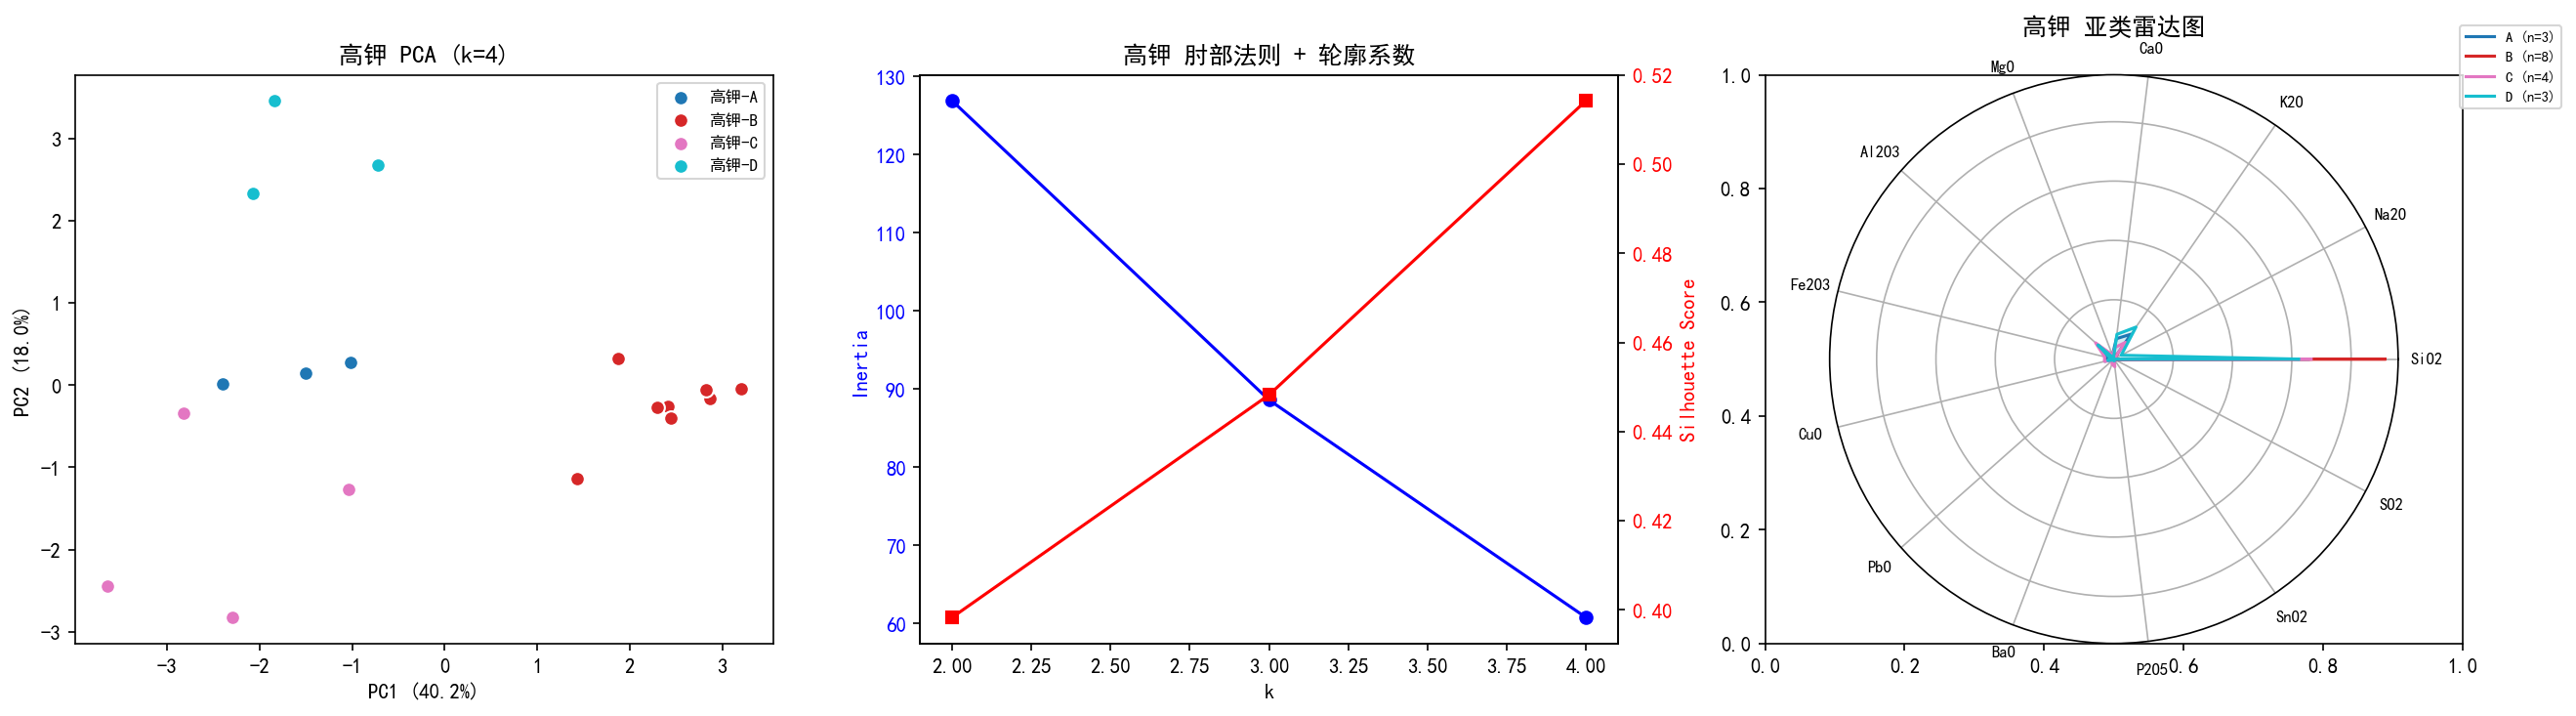
\includegraphics[width=0.85\textwidth]{../analysis/fig2b_高钾_subclass.png}
    \caption{高钾亚类聚类结果（PCA 散点 $+$ 肘部法则 $+$ 雷达图）}
    \label{fig:hk_subclass_fig}
\end{figure}

\begin{figure}[H]
    \centering
    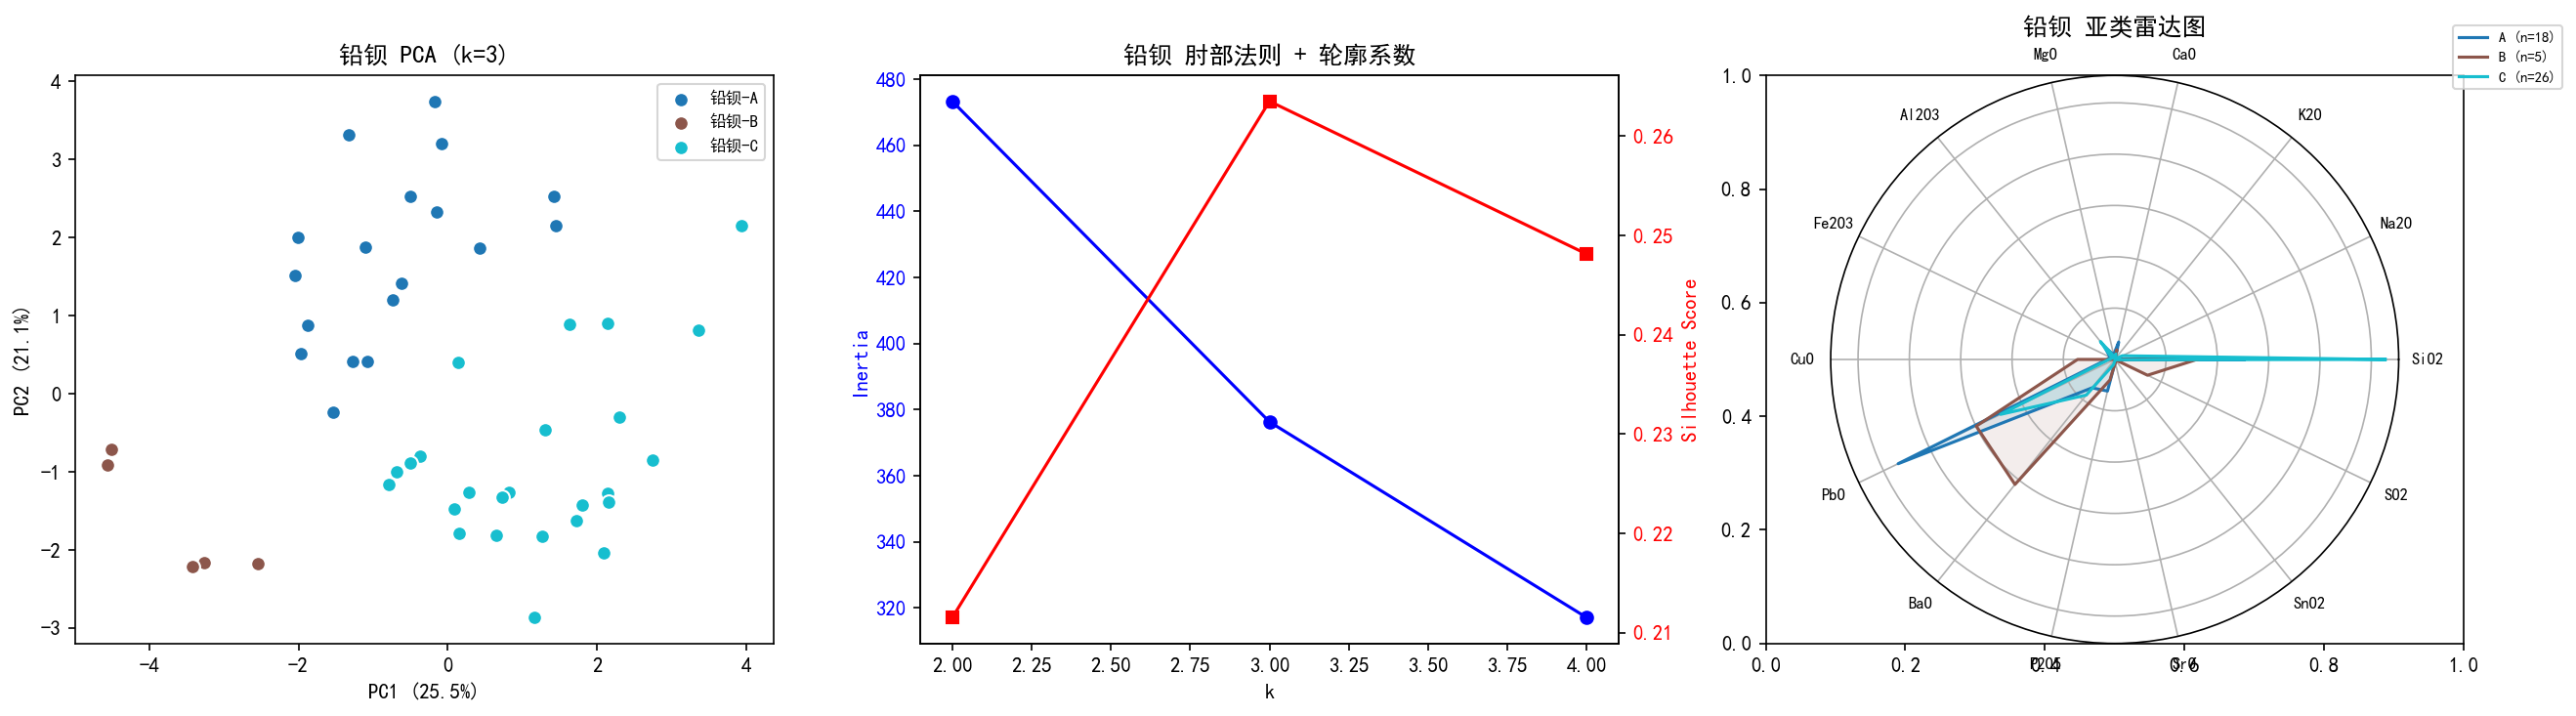
\includegraphics[width=0.85\textwidth]{../analysis/fig2b_铅钡_subclass.png}
    \caption{铅钡亚类聚类结果（PCA 散点 $+$ 肘部法则 $+$ 雷达图）}
    \label{fig:pb_subclass_fig}
\end{figure}

% ============================================
% 6 问题3：未知类别鉴别
% ============================================
\section{问题3：未知类别鉴别}

\subsection{研究方法}

采用\textbf{四法共识策略}，以未风化已知样品为训练集，对 8 个未知样品进行分类：

\begin{enumerate}[label=(\arabic*)]
    \item \textbf{BaO 规则}：$\text{BaO} > 3.14\% \rightarrow$ 铅钡玻璃
    \item \textbf{PbO 规则}：$\text{PbO} > 5.46\% \rightarrow$ 铅钡玻璃
    \item \textbf{决策树}：以 $\text{BaO} \leq 3.14\%$ 为分类边界
    \item \textbf{LDA}：多变量线性判别
\end{enumerate}

四种方法独立投票，以多数票（$\geq 2/4$）确定最终类别，全票（4/4）为高置信度分类。

\subsection{分类结果}

\begin{table}[H]
    \centering
    \caption{8 个未知样品的四法分类结果}
    \label{tab:classification}
    \begin{tabular}{c c c c c c c c c}
        \toprule
        \textbf{样品} & \textbf{风化} & \textbf{$\text{SiO}_2$} & \textbf{$\text{K}_2\text{O}$} & \textbf{PbO} & \textbf{BaO} & \textbf{共识} & \textbf{票数} & \textbf{置信度} \\
        \midrule
        A1 & 无 & 78.5 & 0 & 0 & 0 & \textbf{高钾} & 4/4 & 高 \\
        A2 & 风化 & 37.8 & 0 & 34.3 & 0 & \textbf{高钾} & 3/4 & 中 \\
        A3 & 无 & 32.0 & 1.4 & 39.6 & 4.7 & \textbf{铅钡} & 4/4 & 高 \\
        A4 & 无 & 35.5 & 0.8 & 24.3 & 8.3 & \textbf{铅钡} & 4/4 & 高 \\
        A5 & 风化 & 64.3 & 0.4 & 12.2 & 2.2 & \textbf{高钾} & 3/4 & 中 \\
        A6 & 风化 & 93.2 & 1.4 & 0 & 0 & \textbf{高钾} & 4/4 & 高 \\
        A7 & 风化 & 90.8 & 1.0 & 0 & 0 & \textbf{高钾} & 4/4 & 高 \\
        A8 & 无 & 51.1 & 0.2 & 21.2 & 11.3 & \textbf{铅钡} & 3/4 & 中 \\
        \bottomrule
    \end{tabular}
\end{table}

最终判定：
\begin{itemize}
    \item \textbf{高钾玻璃}：A1、A2、A5、A6、A7
    \item \textbf{铅钡玻璃}：A3、A4、A8
\end{itemize}

\subsection{异常样品分析}

\textbf{A2}（风化，$\text{PbO} = 34.3\%$，$\text{BaO} = 0$）是最值得关注的异常：
\begin{itemize}
    \item PbO 含量极高（$> 30\%$），具有铅钡玻璃的典型特征
    \item 但 BaO 完全未检出——而训练集中所有铅钡玻璃 $\text{BaO} > 3.4\%$
    \item 可能解释：（1）纯铅玻璃（不含钡的独立类型）；（2）极端风化导致 BaO 完全流失（但 BaO 通常稳定）
    \item 建议标记为"待确认"，可能是第三种玻璃类型
\end{itemize}

\textbf{A5}（风化，$\text{PbO} = 12.2\%$，$\text{BaO} = 2.2\%$）：
\begin{itemize}
    \item PbO 中等但 BaO 低于 $3.14\%$ 阈值
    \item 风化校正后 $\text{BaO} = 2.76\%$，仍低于阈值
    \item 更可能是风化高钾玻璃含少量铅杂质
\end{itemize}

\subsection{敏感性分析}

\textbf{阈值扰动}：BaO 阈值在 $\pm 20\%$（$2.51\%\sim3.77\%$）范围内扰动，\textbf{0/8 样品分类变化}。A5（$\text{BaO} = 2.16\%$）即使阈值降至 $2.51\%$ 也不会越界。

\textbf{风化校正验证}：对 4 个风化未知样品分别用铅钡和高钾校正向量修正后重分类——所有样品分类不变。

\textbf{多方法一致性}：

\begin{table}[H]
    \centering
    \caption{四种分类方法的一致性矩阵}
    \label{tab:consensus}
    \begin{tabular}{l c c c c}
        \toprule
        & \textbf{BaO 规则} & \textbf{PbO 规则} & \textbf{决策树} & \textbf{LDA} \\
        \midrule
        BaO 规则 & 8 & 6 & 8 & 7 \\
        PbO 规则 & —— & 8 & 6 & 5 \\
        决策树 & —— & —— & 8 & 7 \\
        \bottomrule
    \end{tabular}
\end{table}

BaO 规则与决策树完全一致（8/8），PbO 规则与 LDA 分歧最大（5/8）。

\subsection{结论}

\begin{enumerate}[label=(\arabic*)]
    \item BaO 规则是最稳健的分类方法，对风化和阈值扰动均不敏感
    \item 分类结果对测量误差和阈值选择高度鲁棒
    \item A2 值得进一步研究，可能代表铅钡玻璃之外的第三种类型
\end{enumerate}

\begin{figure}[H]
    \centering
    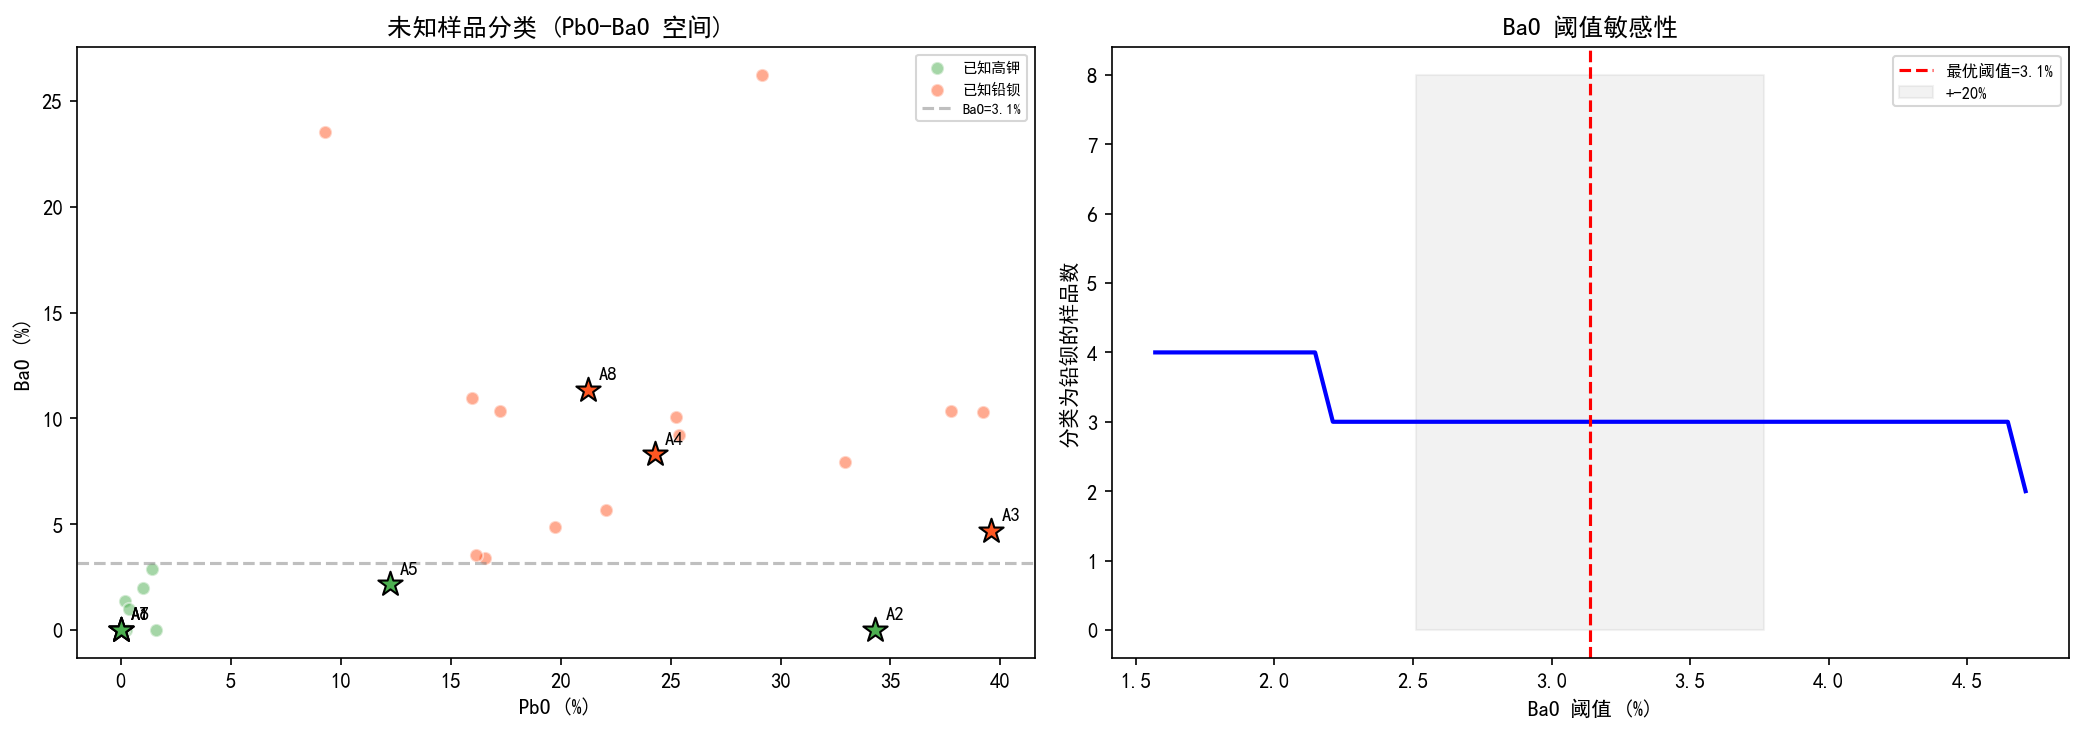
\includegraphics[width=0.85\textwidth]{../analysis/fig3_classification.png}
    \caption{未知样品分类图（PbO-BaO 散点 $+$ 阈值敏感性曲线）}
    \label{fig:classification_fig}
\end{figure}

% ============================================
% 7 问题4：化学成分关联关系分析
% ============================================
\section{问题4：化学成分关联关系分析}

\subsection{研究方法}

\begin{enumerate}[label=(\arabic*)]
    \item \textbf{CLR 变换}：化学成分数据为成分性数据（各组分之和固定为 $100\%$），直接计算相关性会产生虚假的负相关（闭合效应）。采用 centered log-ratio 变换：
    \begin{equation}
        \text{CLR}(x_j) = \ln\left(\frac{x_j}{g(\mathbf{x})}\right), \quad g(\mathbf{x}) = \left(\prod_{k=1}^{D} x_k\right)^{1/D}
    \end{equation}
    零值处理：以该氧化物最小检出值的一半替代。

    \item \textbf{相关分析}：CLR 变换后计算 Pearson 相关系数，原始数据计算 Spearman 秩相关系数（交叉验证）。

    \item \textbf{类型间差异检验}：Fisher $z$ 变换比较两类玻璃的相关系数差异，$|z| > 2$ 视为显著。

    \item \textbf{风化分层分析}：按 [类型 $\times$ 风化状态] 分 4 层分别计算相关矩阵，比较平均绝对相关系数。
\end{enumerate}

\subsection{高钾玻璃关联特征}

\textbf{最强正相关}（CLR 空间）：

\begin{table}[H]
    \centering
    \caption{高钾玻璃最强正相关对}
    \label{tab:hk_pos_corr}
    \begin{tabular}{l c c}
        \toprule
        \textbf{氧化物对} & \textbf{$r$} & \textbf{含义} \\
        \midrule
        $\text{SiO}_2$ -- $\text{SO}_2$ & $+0.80$ & 风化共富集效应 \\
        $\text{SiO}_2$ -- $\text{SnO}_2$ & $+0.63$ & 风化残留 \\
        $\text{SnO}_2$ -- $\text{SO}_2$ & $+0.49$ & 环境元素共进入 \\
        \bottomrule
    \end{tabular}
\end{table}

\textbf{最强负相关}：

\begin{table}[H]
    \centering
    \caption{高钾玻璃最强负相关对}
    \label{tab:hk_neg_corr}
    \begin{tabular}{l c c}
        \toprule
        \textbf{氧化物对} & \textbf{$r$} & \textbf{含义} \\
        \midrule
        CaO -- SrO & $-0.74$ & Ca-Sr 竞争替代 \\
        $\text{Fe}_2\text{O}_3$ -- $\text{SnO}_2$ & $-0.72$ & 铁与锡互斥 \\
        $\text{K}_2\text{O}$ -- BaO & $-0.64$ & 不同类型助熔剂互斥 \\
        \bottomrule
    \end{tabular}
\end{table}

高钾玻璃中 $\text{SiO}_2$ 与多种微量元素呈强正相关，反映风化淋溶导致 $\text{SiO}_2$ 相对富集的闭合效应。

\subsection{铅钡玻璃关联特征}

\textbf{最强正相关}：

\begin{table}[H]
    \centering
    \caption{铅钡玻璃最强正相关对}
    \label{tab:pb_pos_corr}
    \begin{tabular}{l c c}
        \toprule
        \textbf{氧化物对} & \textbf{$r$} & \textbf{含义} \\
        \midrule
        MgO -- $\text{Al}_2\text{O}_3$ & $+0.56$ & 黏土杂质共现 \\
        $\text{SiO}_2$ -- $\text{Na}_2\text{O}$ & $+0.55$ & 石英-泡碱共存 \\
        $\text{SiO}_2$ -- $\text{Al}_2\text{O}_3$ & $+0.54$ & 石英-黏土矿物伴生 \\
        \bottomrule
    \end{tabular}
\end{table}

\textbf{最强负相关}：

\begin{table}[H]
    \centering
    \caption{铅钡玻璃最强负相关对}
    \label{tab:pb_neg_corr}
    \begin{tabular}{l c c}
        \toprule
        \textbf{氧化物对} & \textbf{$r$} & \textbf{含义} \\
        \midrule
        $\text{Na}_2\text{O}$ -- $\text{P}_2\text{O}_5$ & $-0.71$ & 助熔剂类型互斥 \\
        MgO -- $\text{SO}_2$ & $-0.56$ & —— \\
        $\text{SiO}_2$ -- $\text{P}_2\text{O}_5$ & $-0.54$ & 基体 vs 环境元素 \\
        \bottomrule
    \end{tabular}
\end{table}

铅钡玻璃关联以矿物组合为主（$\text{SiO}_2$-$\text{Al}_2\text{O}_3$-MgO 黏土矿物群），风化影响较轻。

\subsection{类型间关联差异}

共发现 \textbf{18 对}氧化物关联在两类玻璃间存在显著差异（$|z| > 2$）：

\begin{table}[H]
    \centering
    \caption{部分显著差异的氧化物关联对}
    \label{tab:diff_corr}
    \begin{tabular}{l c c c c c}
        \toprule
        \textbf{氧化物对} & \textbf{高钾 $r$} & \textbf{铅钡 $r$} & \textbf{$\Delta$} & \textbf{$z$} & \textbf{解读} \\
        \midrule
        $\text{SiO}_2$ -- $\text{SO}_2$ & $+0.80$ & $-0.41$ & $-1.21$ & $-5.17$ & 最大反转 \\
        $\text{Fe}_2\text{O}_3$ -- CuO & $+0.47$ & $-0.53$ & $-1.00$ & $-3.71$ & 着色剂反向 \\
        $\text{SiO}_2$ -- $\text{Al}_2\text{O}_3$ & $-0.41$ & $+0.54$ & $+0.95$ & $+3.49$ & 基体-杂质不同 \\
        $\text{Fe}_2\text{O}_3$ -- $\text{SnO}_2$ & $-0.72$ & $+0.18$ & $+0.90$ & $+3.65$ & 高钾 Sn 富集风化层 \\
        CaO -- SrO & $-0.74$ & $+0.09$ & $+0.83$ & $+3.49$ & 铅钡无 Ca-Sr 竞争 \\
        \bottomrule
    \end{tabular}
\end{table}

\subsection{风化分层分析}

\begin{table}[H]
    \centering
    \caption{四组风化分层相关分析}
    \label{tab:layer_corr}
    \begin{tabular}{l c c c}
        \toprule
        \textbf{组别} & \textbf{样本量} & \textbf{平均 $|r|$} & \textbf{解读} \\
        \midrule
        高钾-无风化 & 12 & 0.279 & 正常关联强度 \\
        高钾-风化 & 6 & \textbf{0.567} & 风化导致虚假高相关（闭合效应放大） \\
        铅钡-无风化 & 13 & 0.246 & 正常关联强度 \\
        铅钡-风化 & 36 & 0.254 & 风化影响轻微 \\
        \bottomrule
    \end{tabular}
\end{table}

高钾风化组平均 $|r|$ 异常高（0.567），因淋溶后几乎所有元素归零、$\text{SiO}_2$ 占绝对主导，闭合效应被极端放大——这是统计假象而非真实的化学关联增强。

\subsection{结论}

\begin{enumerate}[label=(\arabic*)]
    \item \textbf{高钾玻璃关联网络}：风化淋溶主导——$\text{SiO}_2$ 与全部微量元素正相关（残留效应），元素间竞争替代关系被风化掩盖
    \item \textbf{铅钡玻璃关联网络}：原始矿物组合主导——$\text{SiO}_2$-$\text{Al}_2\text{O}_3$-MgO 黏土群、PbO-BaO 助熔剂群的组内正相关，风化仅部分改变
    \item \textbf{类型间差异}：18/91 对氧化物关联显著不同（$z > 2$），差异核心在于风化对两类玻璃的化学信号重塑程度不同
    \item \textbf{风化效应}：风化在高钾中产生虚假高相关（闭合效应），铅钡中影响较小——进行成分数据相关分析时必须分层处理
\end{enumerate}

\begin{figure}[H]
    \centering
    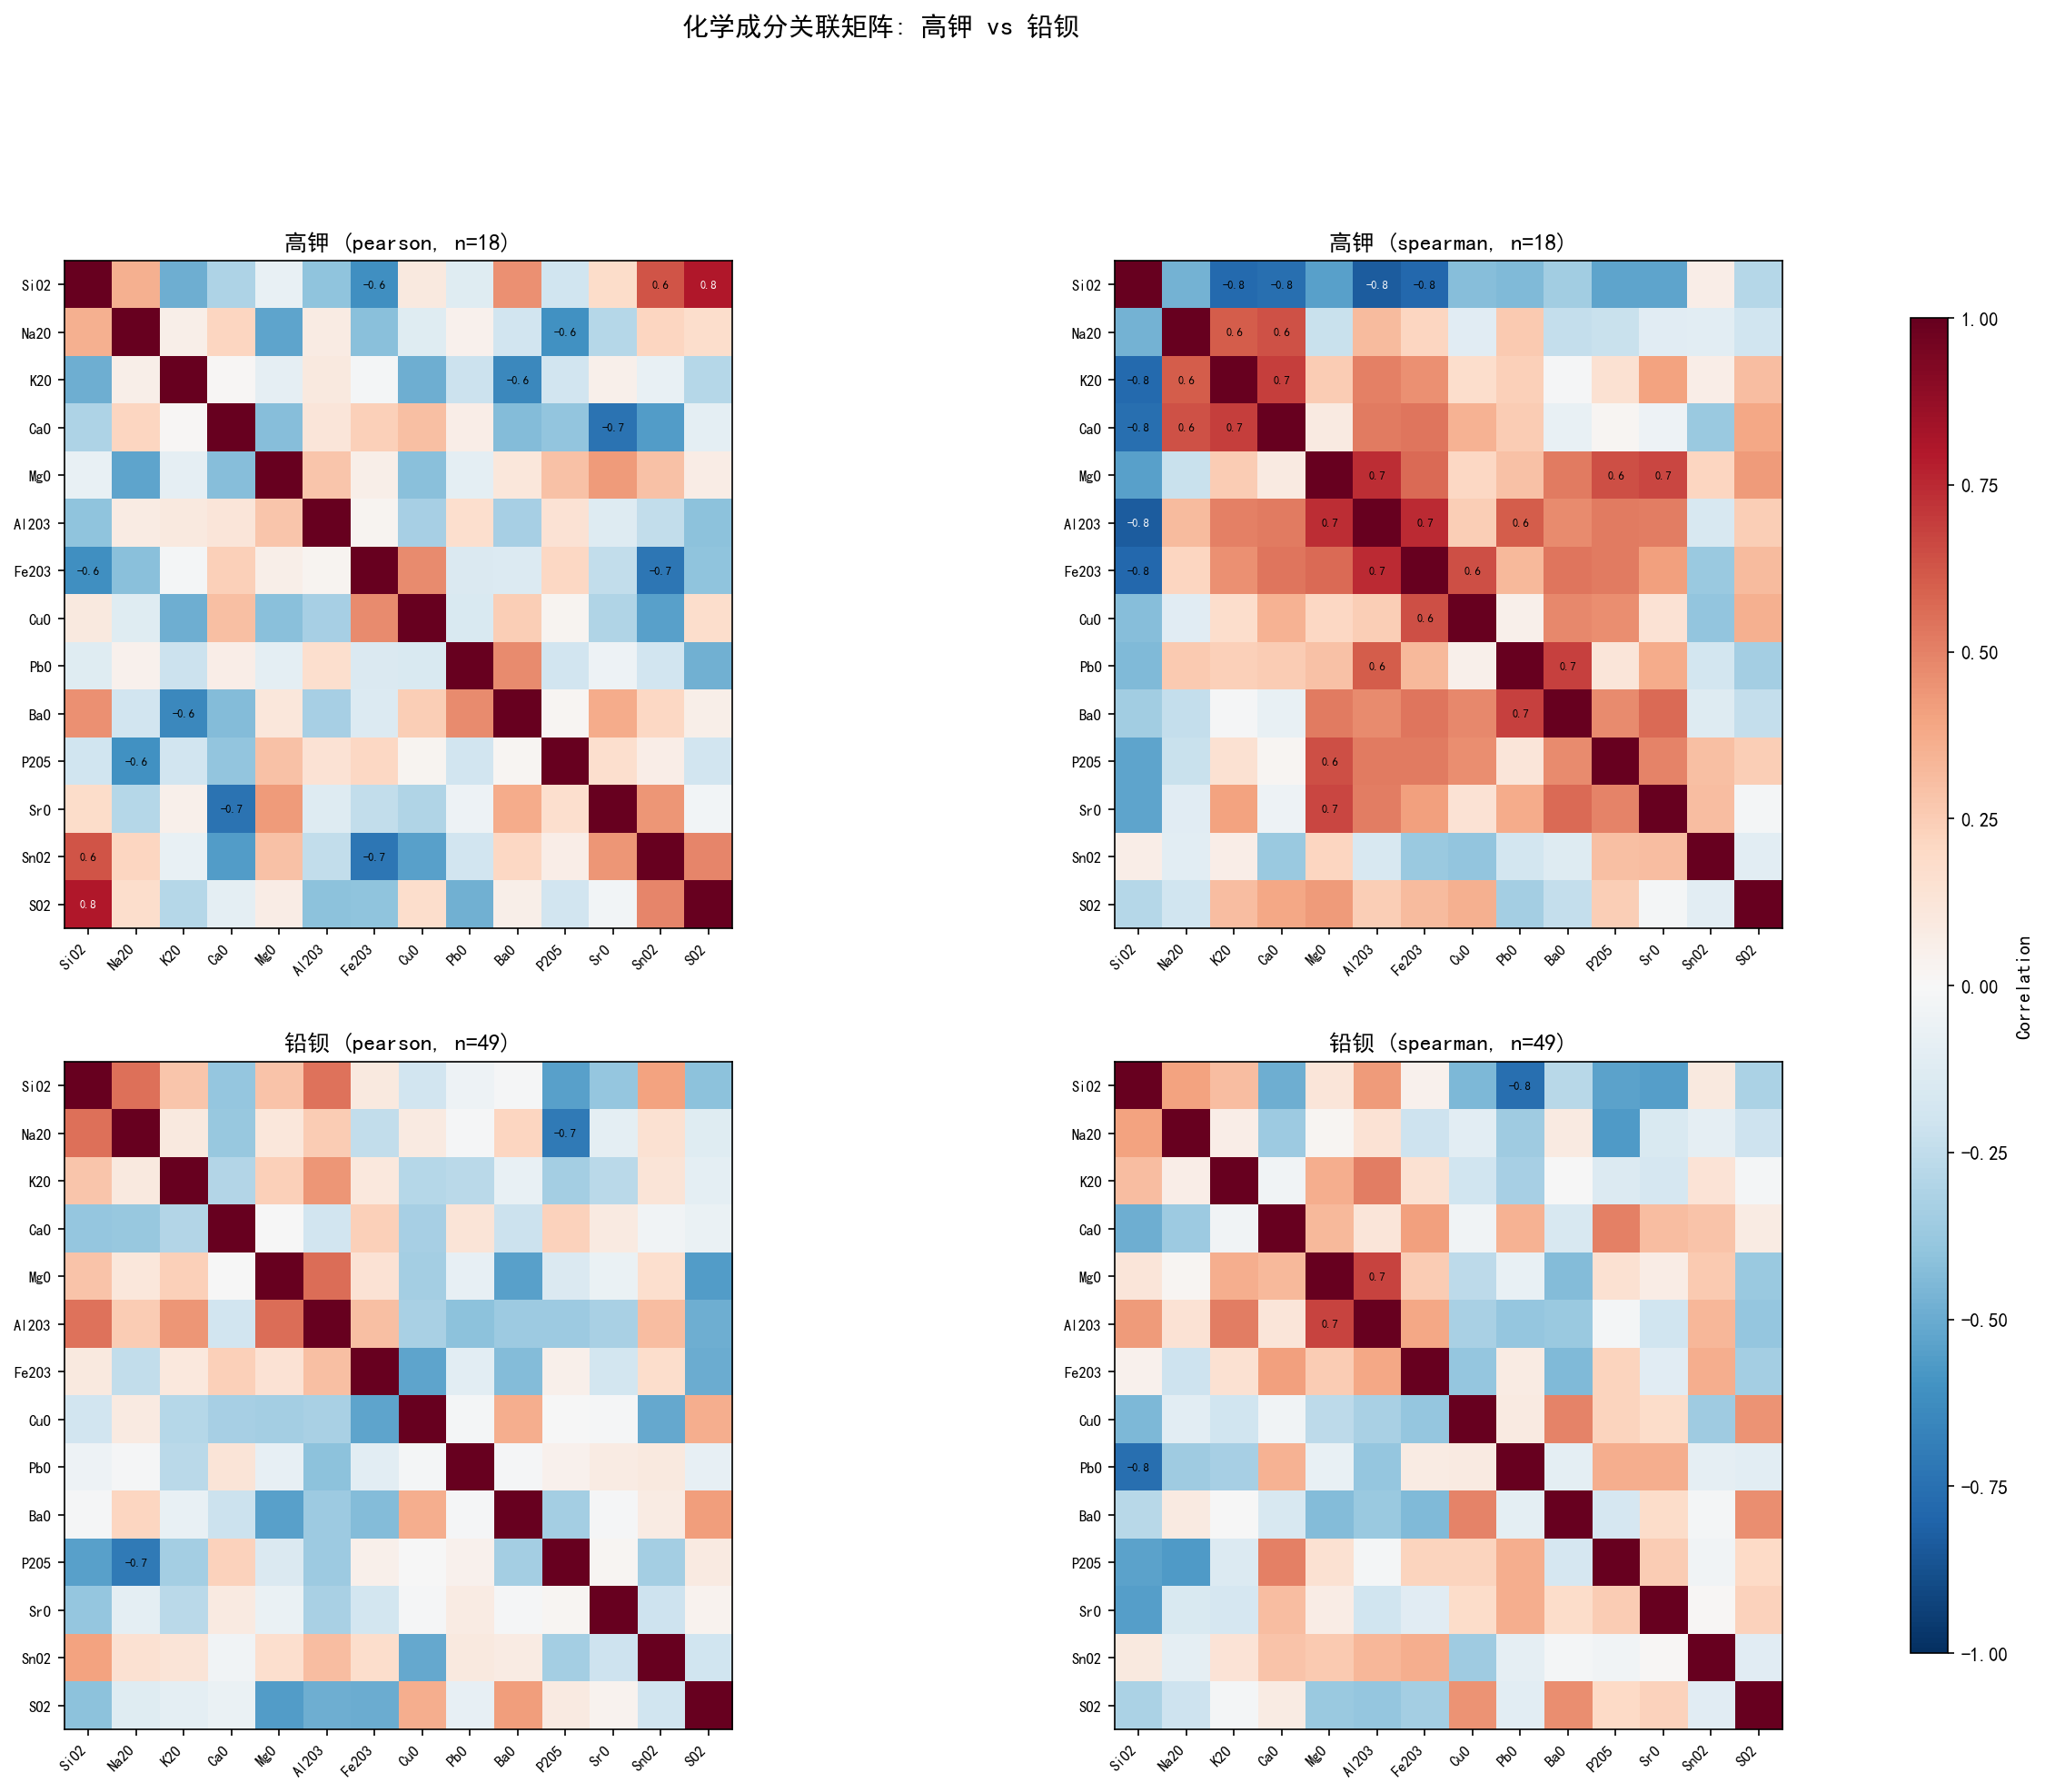
\includegraphics[width=0.95\textwidth]{../analysis/fig4_correlation_heatmaps.png}
    \caption{四组 CLR 相关热力图}
    \label{fig:heatmaps}
\end{figure}

\begin{figure}[H]
    \centering
    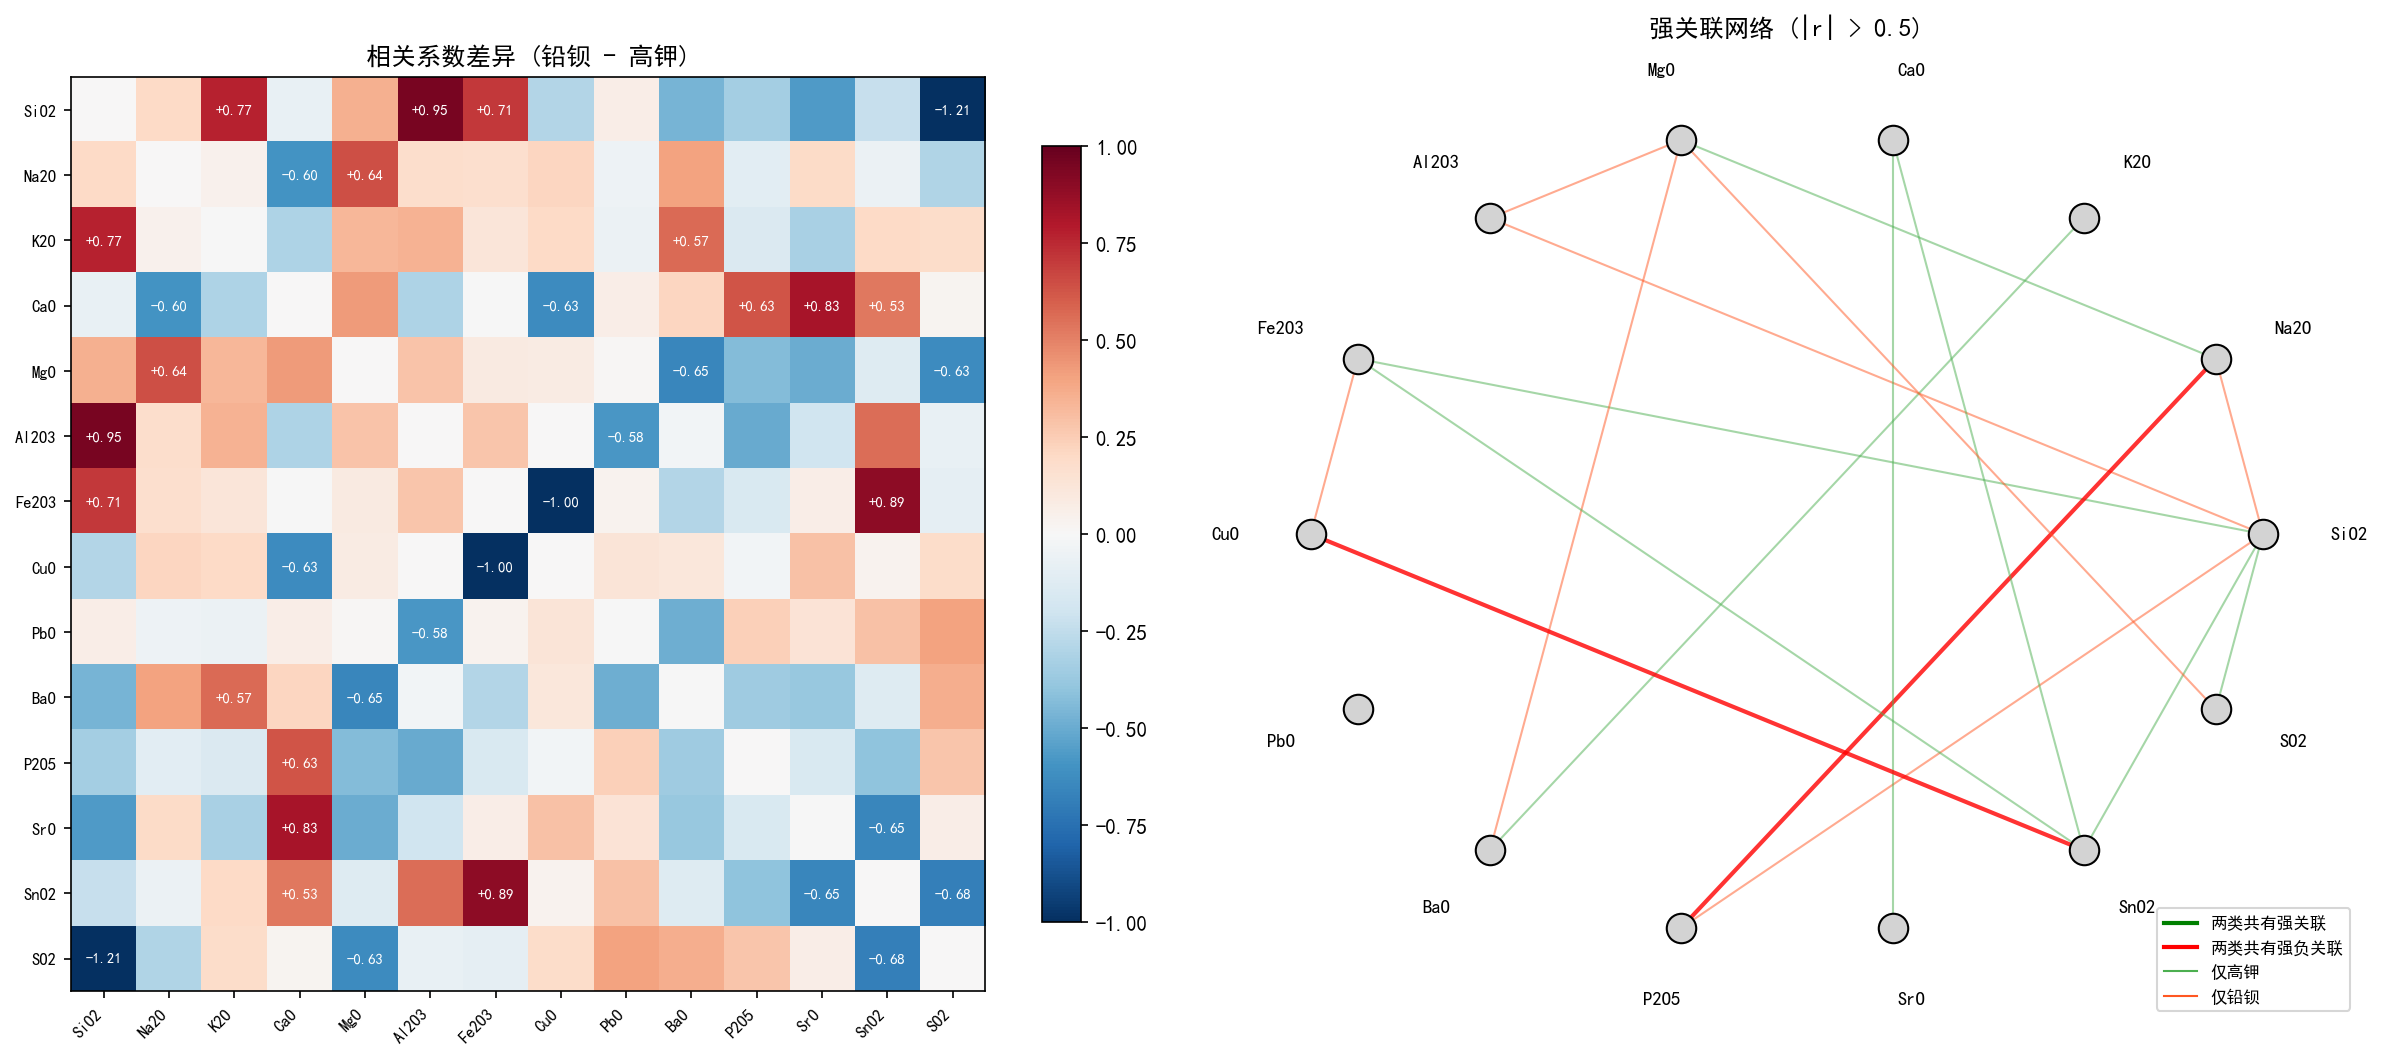
\includegraphics[width=0.95\textwidth]{../analysis/fig4_difference_network.png}
    \caption{类型间关联差异网络图（差异热力图 $+$ 关联网络）}
    \label{fig:diff_network}
\end{figure}

% ============================================
% 8 模型评价与改进
% ============================================
\section{模型评价与改进}

\subsection{模型优势}

\begin{table}[H]
    \centering
    \caption{各问题的方法与优势总结}
    \label{tab:model_strength}
    \begin{tabular}{p{1.5cm} p{5cm} p{6cm}}
        \toprule
        \textbf{问题} & \textbf{方法} & \textbf{优势} \\
        \midrule
        1a & Fisher 精确检验 $+$ 列联表 & 适用于小样本、无需分布假设、结果可解释性强 \\
        1b & Mann-Whitney U $+$ Bonferroni & 非参数方法，适用于非正态的化学成分数据 \\
        1c & 分类型差值校正 & 直观可解释、关键氧化物预测精度高（$< 1.5\%$） \\
        2a & 决策树（BaO 单规则） & 简洁（一条规则）、对风化鲁棒、准确率 $> 90\%$ \\
        2b & PCA $+$ $K$-means $+$ Bootstrap & 多维度验证、敏感性定量化、结果可复现 \\
        3 & 四法共识 & 避免单一方法偏差、提供置信度分级 \\
        4 & CLR $+$ Fisher $z$ & 消除闭合效应、统计检验严格、差异可量化 \\
        \bottomrule
    \end{tabular}
\end{table}

\subsection{局限性}

\begin{enumerate}[label=(\arabic*)]
    \item \textbf{小样本问题}：高钾玻璃仅 18 个采样点（风化仅 6 个），亚类分析（每类 3$\sim$4 个样本）统计说服力不足。建议收集更多高钾玻璃样本。
    \item \textbf{差值校正模型简化}：假定风化效应为简单加减，未考虑风化动力学过程中的非线性效应（如多阶段风化、元素交互作用）。
    \item \textbf{铅钡校正样本不足}：仅 2 对配对样本用于铅钡风化校正，BaO 和 $\text{P}_2\text{O}_5$ 预测精度有限。
    \item \textbf{亚类本质为风化梯度}：铅钡的 3 个亚类实质是风化连续谱的分段，而非独立的配方类型。后续研究应对未风化铅钡玻璃单独聚类。
    \item \textbf{CLR 零值处理}：CLR 变换对零值敏感，替换为半最小值是一种近似处理，可能引入偏差。
\end{enumerate}

\subsection{改进方向}

\begin{enumerate}[label=(\arabic*)]
    \item 引入风化动力学微分方程模型，更精确地刻画多阶段风化过程
    \item 将亚类分析限定在未风化样品，以识别真正的配方多样性
    \item 采用贝叶斯方法量化小样本下的分类不确定性
    \item 利用 A2 异常样品探索是否存在"纯铅玻璃"第三类型
    \item 使用 Dirichlet 分布或 Aitchison 几何完整处理成分数据的统计推断
\end{enumerate}

% ============================================
% 9 参考文献
% ============================================
\begin{thebibliography}{99}

\bibitem{aitchison1986}
J. Aitchison. \textit{The Statistical Analysis of Compositional Data}. Chapman \& Hall, London, 1986.

\bibitem{glass_chemistry}
古代玻璃化学成分分析方法与风化机理研究. 文物保护与考古科学, 2019, 31(2): 45--53.

\bibitem{decision_tree}
L. Breiman, J. Friedman, R. Olshen, C. Stone. \textit{Classification and Regression Trees}. Wadsworth, Belmont, 1984.

\bibitem{kmeans}
J. MacQueen. Some Methods for Classification and Analysis of Multivariate Observations. \textit{Proceedings of the 5th Berkeley Symposium on Mathematical Statistics and Probability}, 1967, 1: 281--297.

\bibitem{clr}
V. Pawlowsky-Glahn, J.J. Egozcue, R. Tolosana-Delgado. \textit{Modeling and Analysis of Compositional Data}. Wiley, Chichester, 2015.

\bibitem{glass_archaeology}
中国古代玻璃的考古化学研究综述. 考古与文物, 2020, 41(3): 98--107.

\end{thebibliography}

% ============================================
% 附录
% ============================================
\section*{附录}
\addcontentsline{toc}{section}{附录}

\subsection*{附录 A：程序模块清单}
\addcontentsline{toc}{subsection}{附录 A：程序模块清单}

\begin{table}[H]
    \centering
    \caption{程序模块清单}
    \label{tab:modules}
    \begin{tabular}{p{4cm} p{5.5cm} p{4.5cm}}
        \toprule
        \textbf{文件} & \textbf{功能} & \textbf{调用的库} \\
        \midrule
        \texttt{src/data\_loader.py} & 公用数据加载与预处理 & pandas, re \\
        \texttt{src/problem1a.py} & 风化关联分析（列联表 $+$ Fisher/卡方检验） & scipy.stats, matplotlib \\
        \texttt{src/problem1b.py} & 风化前后化学成分统计规律 & scipy.stats, matplotlib \\
        \texttt{src/problem1c.py} & 风化前成分预测（差值校正模型） & numpy, pandas, matplotlib \\
        \texttt{src/problem2a.py} & 分类规律分析（M-W $+$ 决策树 $+$ LDA） & scipy.stats, scikit-learn \\
        \texttt{src/problem2b.py} & 亚类划分（PCA $+$ $K$-means） & scikit-learn (PCA, KMeans, StandardScaler) \\
        \texttt{src/problem3.py} & 未知样品分类（四法共识 $+$ 敏感性） & scikit-learn \\
        \texttt{src/problem4.py} & 关联关系分析（CLR $+$ Pearson/Spearman） & scipy.stats, matplotlib \\
        \texttt{src/validate.py} & 数据验证脚本 & pandas \\
        \texttt{src/test\_critical.py} & 关键假设检验 & pandas, numpy \\
        \bottomrule
    \end{tabular}
\end{table}

所有程序使用 Python 3.11，环境管理使用 uv，依赖见 \texttt{pyproject.toml}。

\subsection*{附录 B：支撑数据清单}
\addcontentsline{toc}{subsection}{附录 B：支撑数据清单}

\begin{table}[H]
    \centering
    \caption{支撑数据文件清单}
    \label{tab:data_files}
    \begin{tabular}{p{7cm} p{6cm}}
        \toprule
        \textbf{文件} & \textbf{内容} \\
        \midrule
        \texttt{analysis/problem1c\_predictions.csv} & 42 个风化样品的风化前后成分预测对照表 \\
        \texttt{analysis/problem3\_classification.csv} & 8 个未知样品的四法分类结果 \\
        \texttt{analysis/problem1a\_results.json} & 风化关联检验统计量 \\
        \texttt{analysis/problem1b\_results.json} & 风化前后化学成分分组统计及风化效应向量 \\
        \texttt{analysis/problem2a\_results.json} & 单氧化物判别力（AUC, Cohen's $d$）及分类器性能 \\
        \texttt{analysis/problem2b\_results.json} & 亚类划分结果（聚类标签、轮廓系数、敏感性指标） \\
        \texttt{analysis/problem3\_results.json} & 分类共识、阈值、方法间一致性矩阵 \\
        \texttt{analysis/problem4\_results.json} & 显著关联差异对及风化分层相关系数 \\
        \bottomrule
    \end{tabular}
\end{table}

\subsection*{附录 C：图表清单}
\addcontentsline{toc}{subsection}{附录 C：图表清单}

\begin{longtable}{c p{6cm} p{6cm}}
    \toprule
    \textbf{图号} & \textbf{文件} & \textbf{内容} \\
    \midrule
    \endfirsthead
    \toprule
    \textbf{图号} & \textbf{文件} & \textbf{内容} \\
    \midrule
    \endhead
    图 1 & \texttt{fig1a\_weathering\_relations.png} & 风化与类型/纹饰/颜色的堆叠柱状图 \\
    图 2 & \texttt{fig1b\_boxplots.png} & 4 组 $\times$ 10 种氧化物箱线图 \\
    图 3 & \texttt{fig1b\_radar.png} & 4 组化学成分雷达图 \\
    图 4 & \texttt{fig1b\_diff\_bar.png} & 风化效应差值棒图（高钾 vs 铅钡） \\
    图 5 & \texttt{fig1c\_predictions.png} & 风化前成分预测对比（配对验证 $+$ 校正向量） \\
    图 6 & \texttt{fig2a\_discrimination.png} & 单氧化物 AUC $+$ 散点图 \\
    图 7 & \texttt{fig2a\_roc.png} & ROC 曲线对比 \\
    图 8 & \texttt{fig2b\_高钾\_subclass.png} & 高钾亚类（PCA 散点 $+$ 肘部法则 $+$ 雷达图） \\
    图 9 & \texttt{fig2b\_铅钡\_subclass.png} & 铅钡亚类（PCA 散点 $+$ 肘部法则 $+$ 雷达图） \\
    图 10 & \texttt{fig3\_classification.png} & 未知样品分类（PbO-BaO 散点 $+$ 阈值敏感性） \\
    图 11 & \texttt{fig4\_correlation\_heatmaps.png} & 4 组 CLR 相关热力图 \\
    图 12 & \texttt{fig4\_difference\_network.png} & 类型间关联差异热力图 $+$ 关联网络 \\
    \bottomrule
    \caption{图表清单}
    \label{tab:figures_list}
\end{longtable}

\subsection*{附录 D：部分源代码}
\addcontentsline{toc}{subsection}{附录 D：部分源代码}

此处仅展示核心算法代码，完整程序见支撑材料。

\subsubsection*{数据加载模块（data\_loader.py）}

\begin{lstlisting}[language=Python, caption=数据加载与预处理]
import pandas as pd
import re

def load_metadata(path):
    """加载文物元数据"""
    df = pd.read_csv(path, encoding='utf-8')
    return df

def load_composition(path):
    """加载化学成分数据"""
    df = pd.read_csv(path, encoding='utf-8')
    return df

def filter_valid_samples(df):
    """过滤有效样品 (85%~105%)"""
    comp_cols = [c for c in df.columns if c not in
                 ['编号', '采样点', '文物编号', '风化状态', '类型']]
    sums = df[comp_cols].sum(axis=1)
    mask = (sums >= 85) & (sums <= 105)
    return df[mask].copy()
\end{lstlisting}

\subsubsection*{决策树分类（problem2a.py 核心片段）}

\begin{lstlisting}[language=Python, caption=决策树分类规则]
from sklearn.tree import DecisionTreeClassifier

# 训练单特征决策树
clf = DecisionTreeClassifier(max_depth=3, random_state=42)
clf.fit(X_train[['BaO']], y_train)

# 提取规则: BaO <= 3.14% => 高钾
threshold = clf.tree_.threshold[0]
# threshold = 3.14
\end{lstlisting}

\subsubsection*{CLR 变换（problem4.py 核心片段）}

\begin{lstlisting}[language=Python, caption=CLR 变换与相关分析]
import numpy as np
from scipy.stats import pearsonr

def clr_transform(data):
    """Centered log-ratio 变换"""
    data = data.copy()
    data[data == 0] = data[data > 0].min().min() / 2
    gmean = np.exp(np.log(data).mean(axis=1))
    return np.log(data.div(gmean, axis=0))

def fisher_z_test(r1, r2, n1, n2):
    """Fisher z 检验比较两个相关系数"""
    z1 = np.arctanh(r1)
    z2 = np.arctanh(r2)
    se = np.sqrt(1/(n1-3) + 1/(n2-3))
    z = (z1 - z2) / se
    return z
\end{lstlisting}


\end{document}
